\documentclass[a4paper, 11pt]{article}
\usepackage[utf8]{inputenc} % Change according your file encoding
\usepackage{graphicx}
\usepackage{url}

%opening
\title{Seminar Report: Paxy}
\author{Maria Gabriela Valdes and Victoria Beleuta}
\date{\today{}}

\begin{document}

\maketitle

\section{Introduction}

This assignment gave us the opportunity to learn and implement the \textit{Paxos} algorithm. This algorithm is a protocol for solving consensus between processes in a distributed system. Consensus consists in agreeing on a proposed value among a group of participants. In this particular case, we have a set of \textit{Proposers} that propose different values, to a set of \textit{Acceptors} until a single and unique value is agreed between all \textit{Proposers} and \textit{Acceptors}.

\section{Work done}

We have completed the code files provided to correctly implement the algorithm. Our source code consists of two folders: \textit{src} and \textit{src-sep}. The first one contains the erlang files implementig the Paxos algorithm with both proposers and acceptors starting in the same instance. The folder \textit{src-sep} we have modules to give the possibility to start the proposers in one machine and the acceptors in a different machine.

\section{Experiments}

First we run an experiment in the same machine with 3 proposers and 5 acceptors. After compiling the code files located in \textit{src} and running the paxy module \textit{paxy:start([200,200,200])}. Proposer 0, \textit{willard} proposes color \textit{blue}, and in round 2, the acceptors voted for \textit{kilgore} and decided on color \textit{blue}.\\
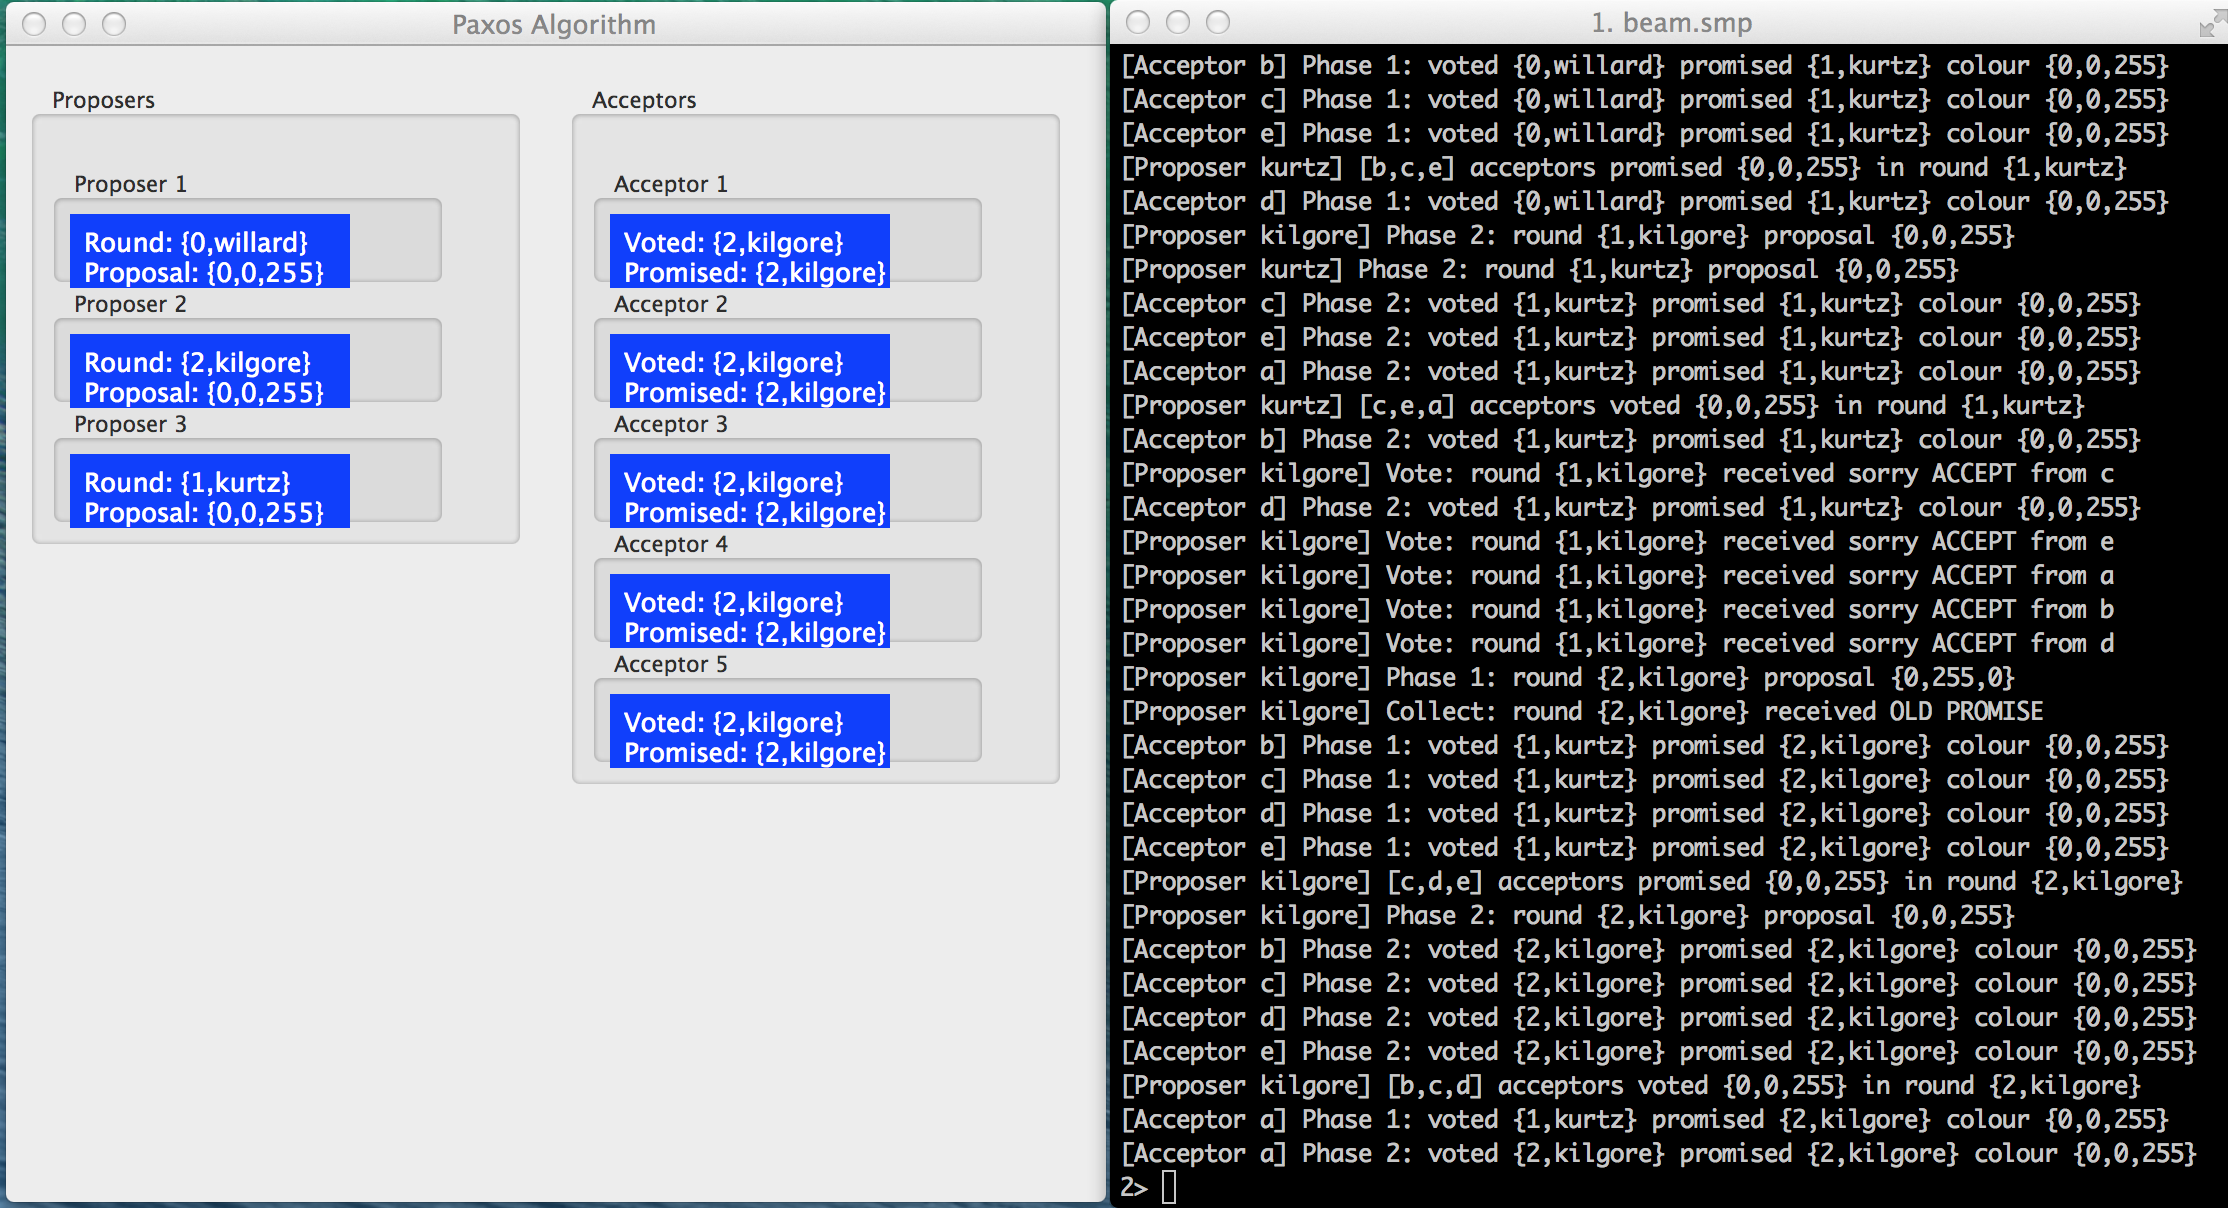
\includegraphics[scale=0.35]{images/exp0.png} \\\\

\textbf{i)} In this experiment we delay \textit{prepare} messages and we see that the algorithm terminates even with the delays shown in the trace.\\
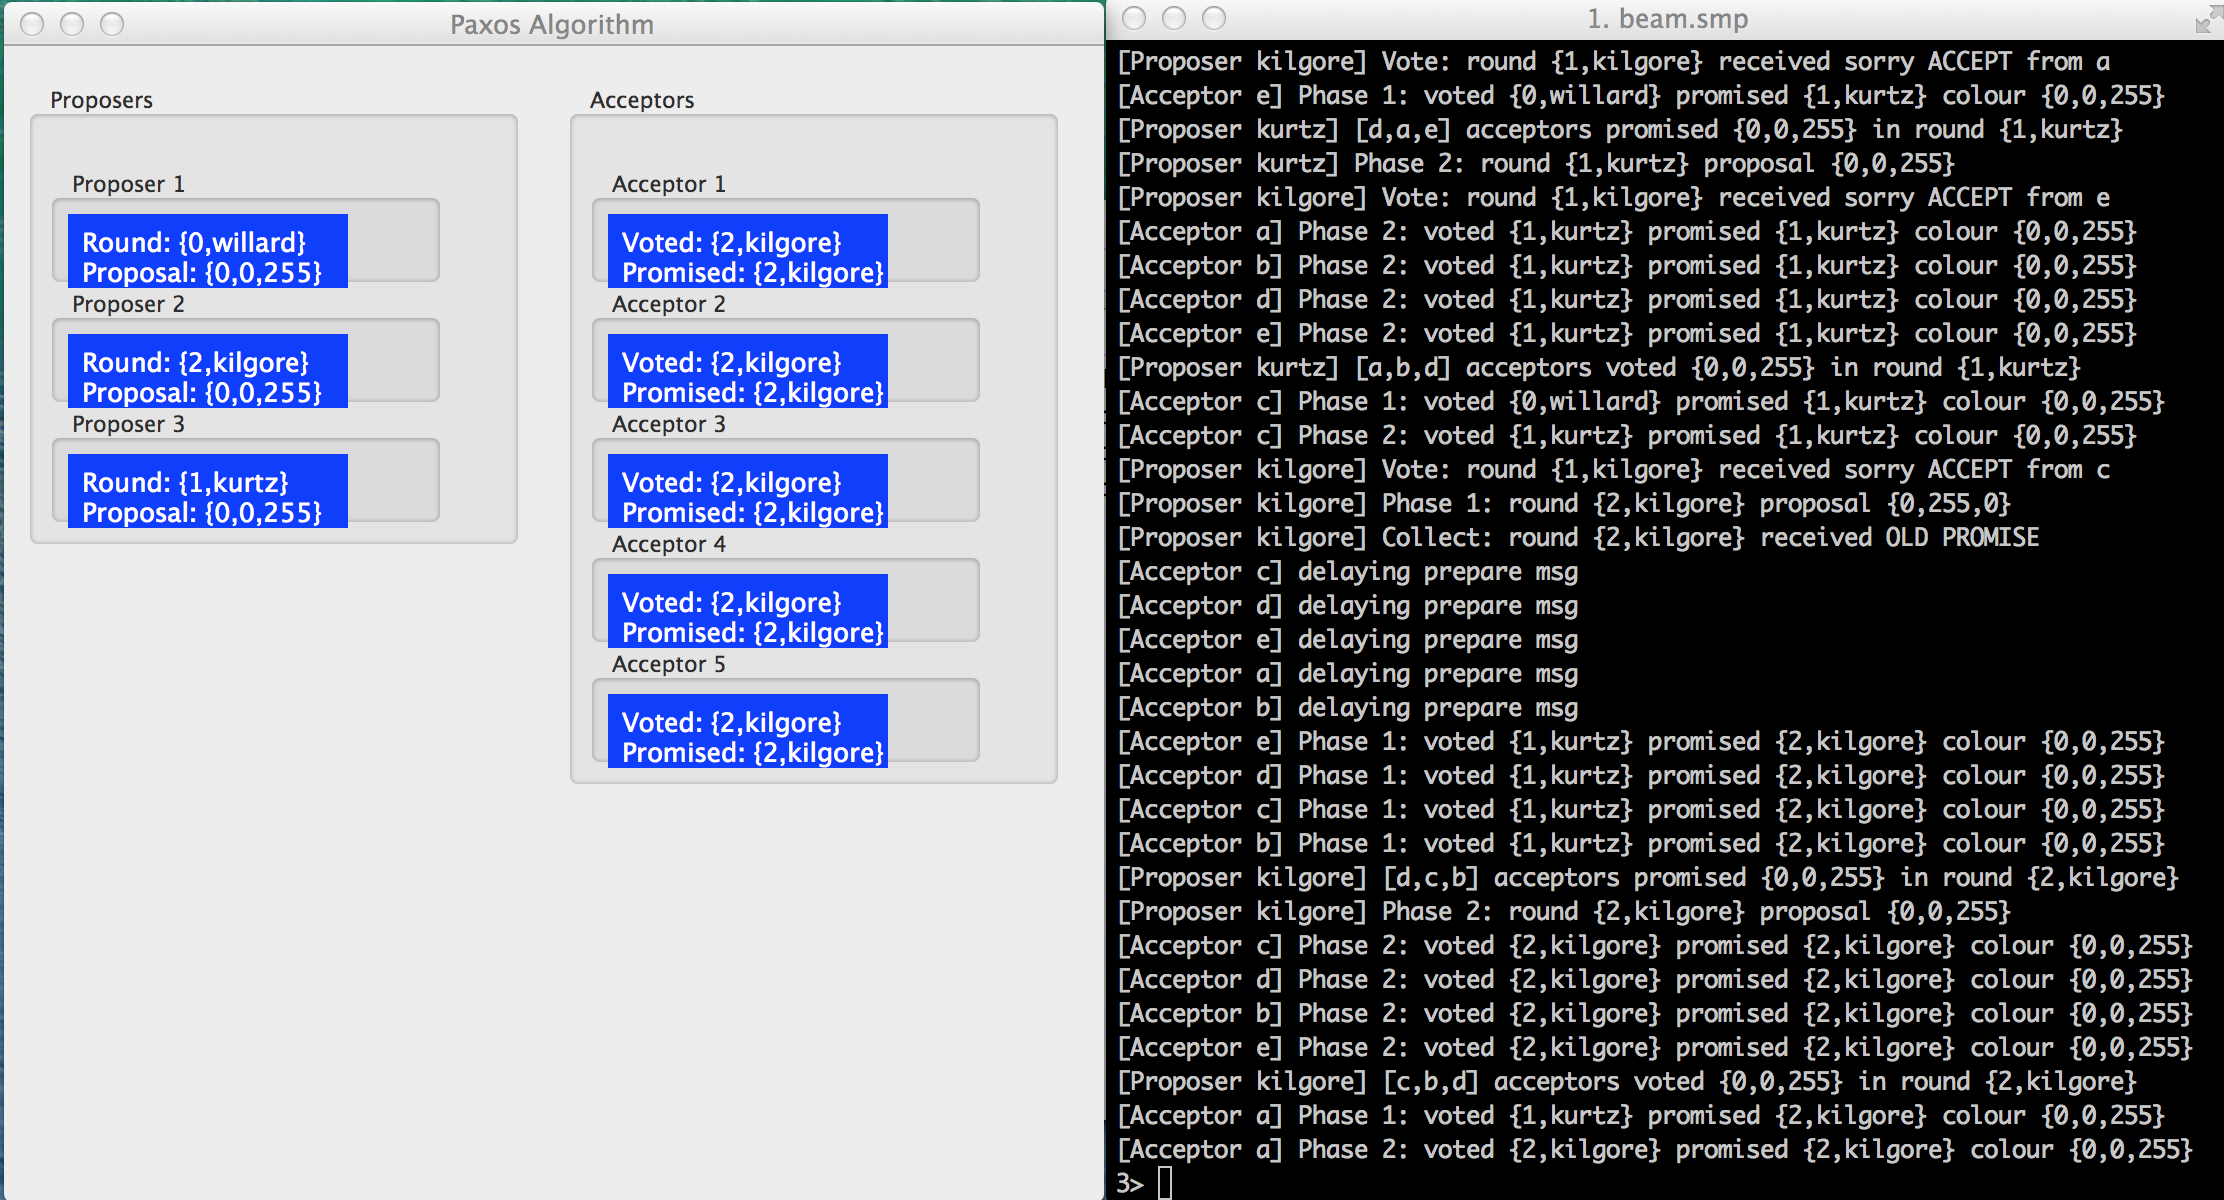
\includegraphics[scale=0.35]{images/exp1.png} \\\\
\newpage
Now we add delays before the \textit{accept} messages, the algorithm terminates voting in round 2 for \textit{kilgore} and color \textit{blue}.\\
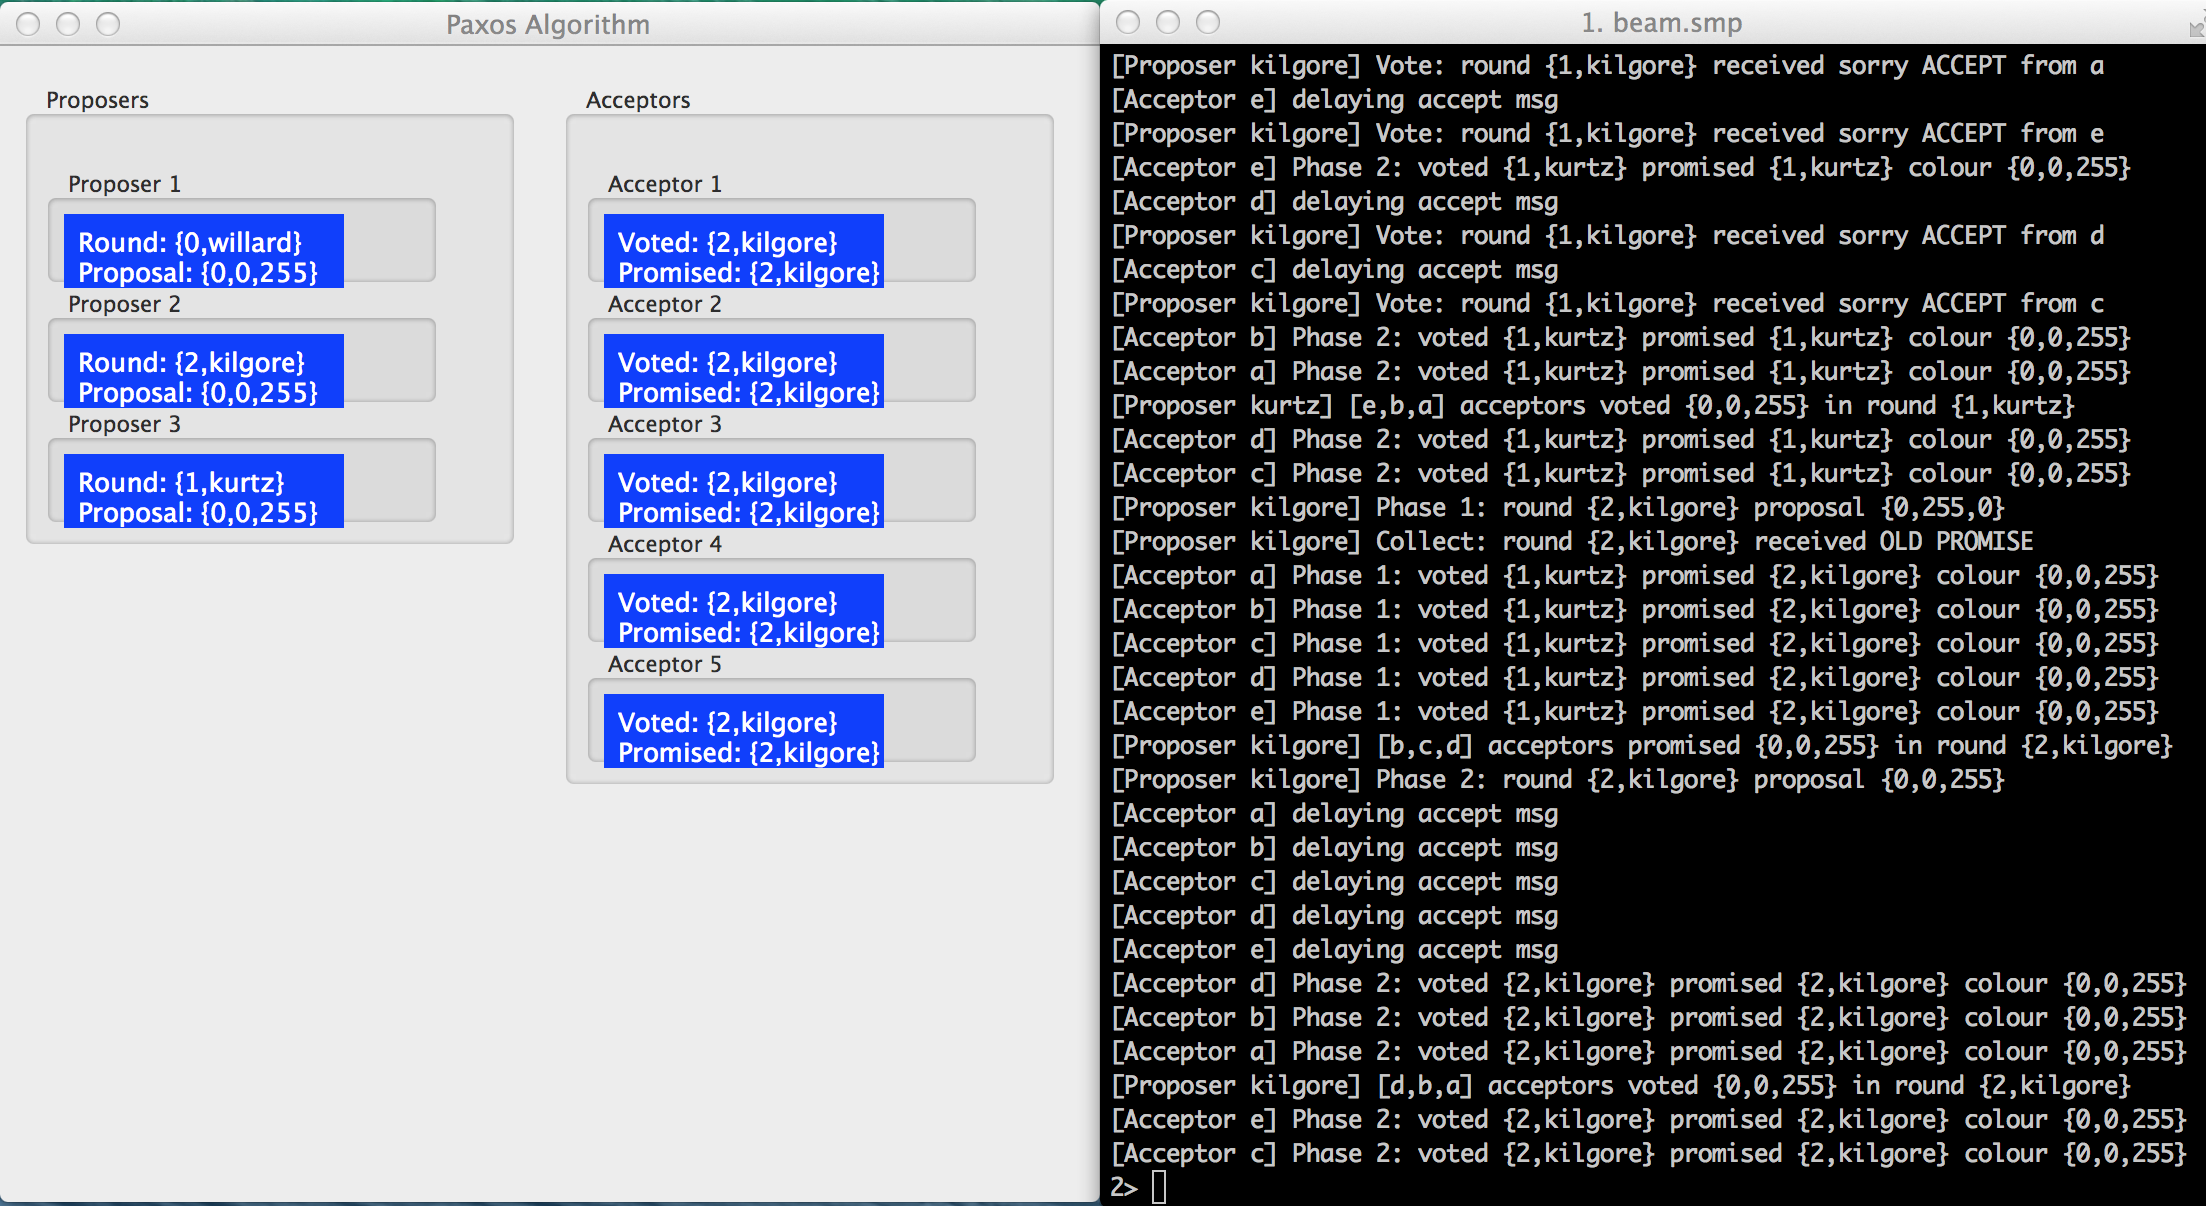
\includegraphics[scale=0.35]{images/exp2.png} \\\\
Lastly, we add delays both before \textit{prepare} and \textit{accept} messages and the acceptors reach the same consensus again.\\
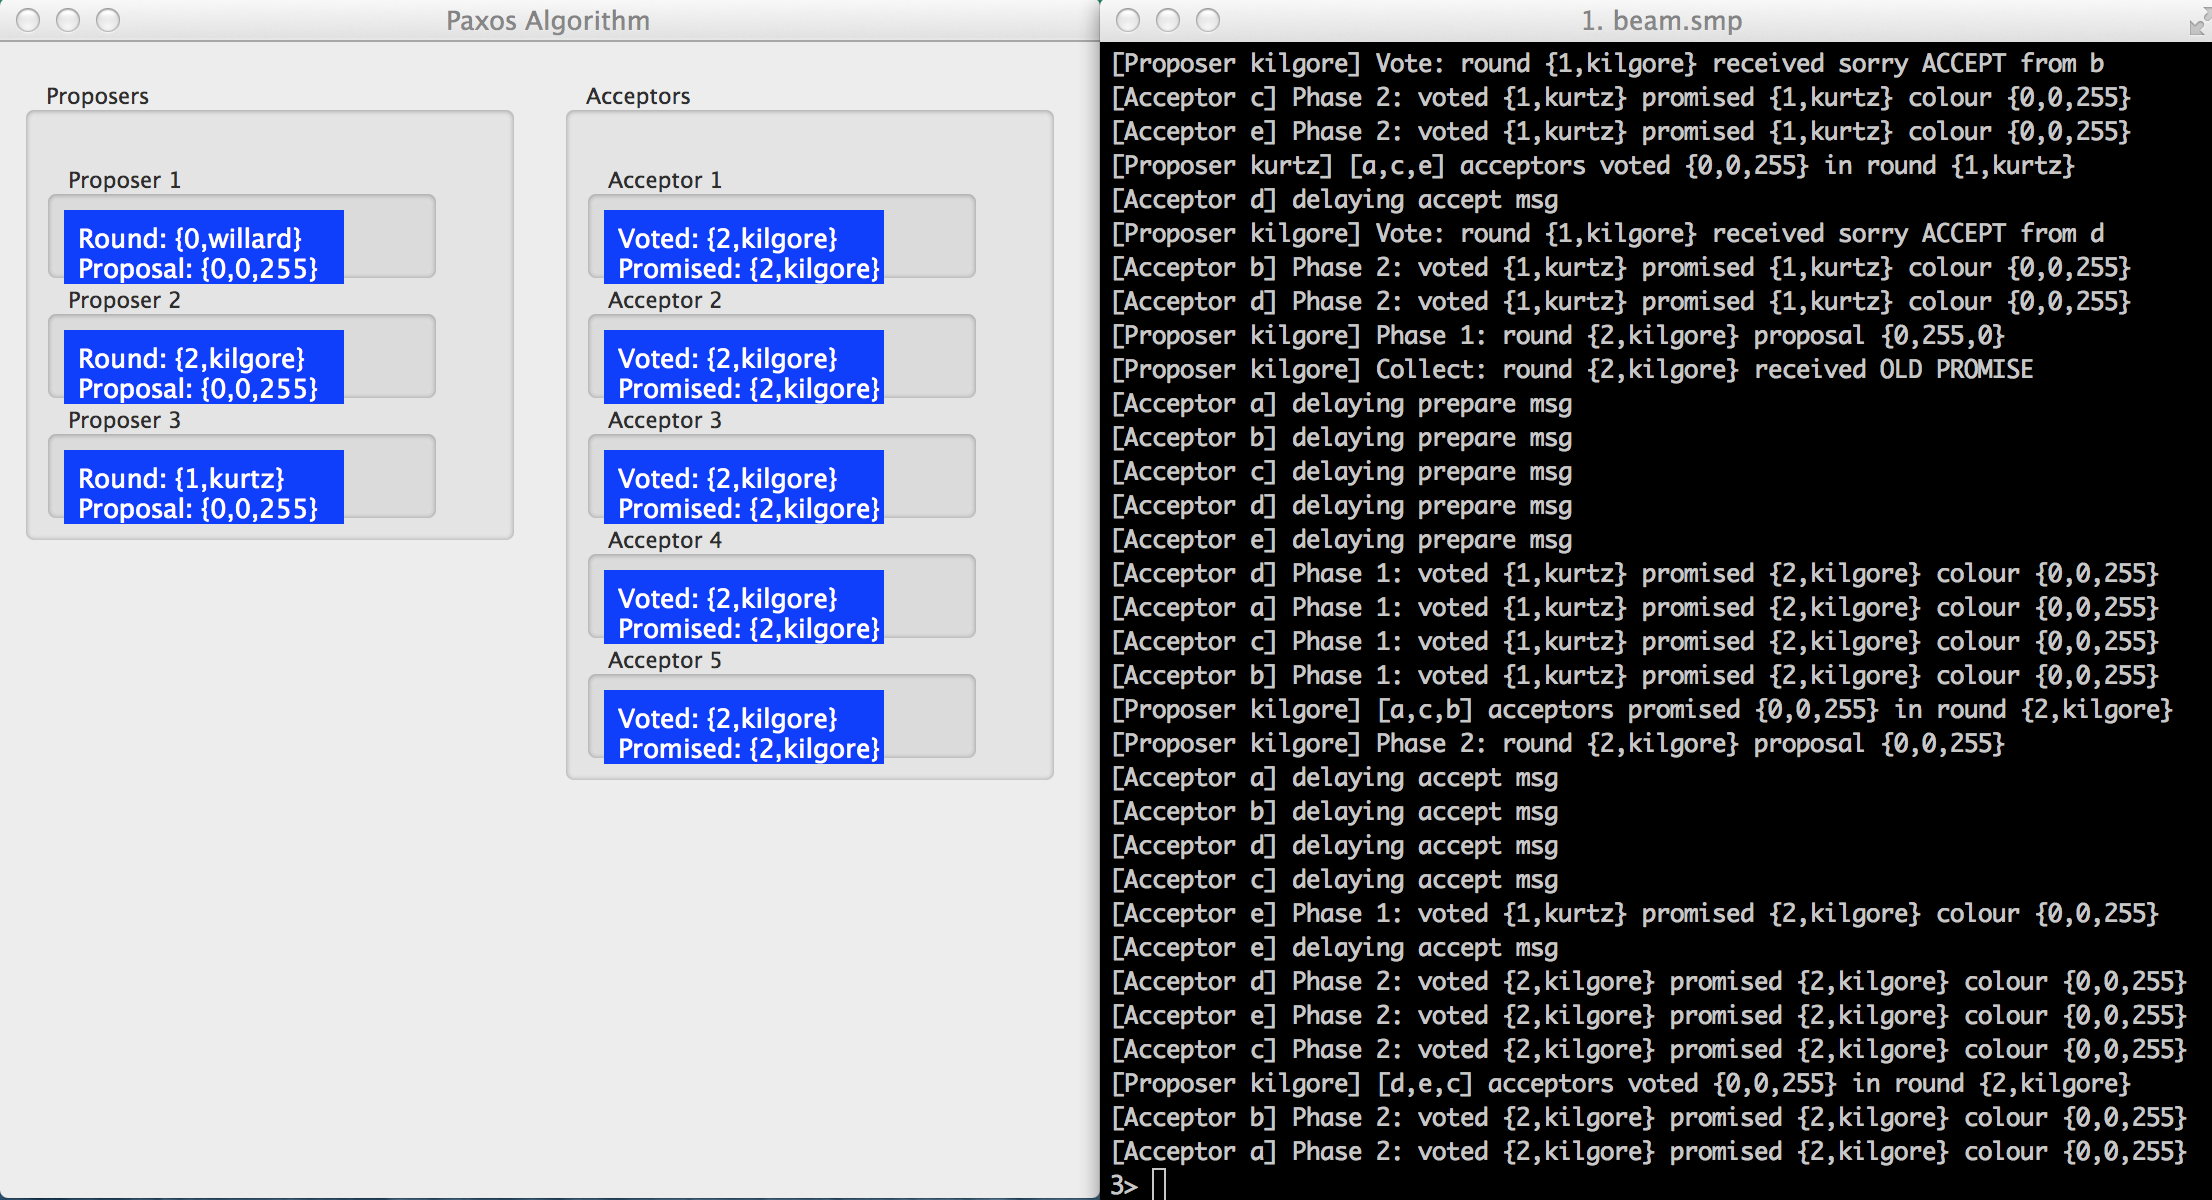
\includegraphics[scale=0.35]{images/exp3.png} \\\\
\newpage
\textbf{ii)} We stop sending \textit{sorry} messages to the processor and we run the experiment to try to reach a consensus.\\
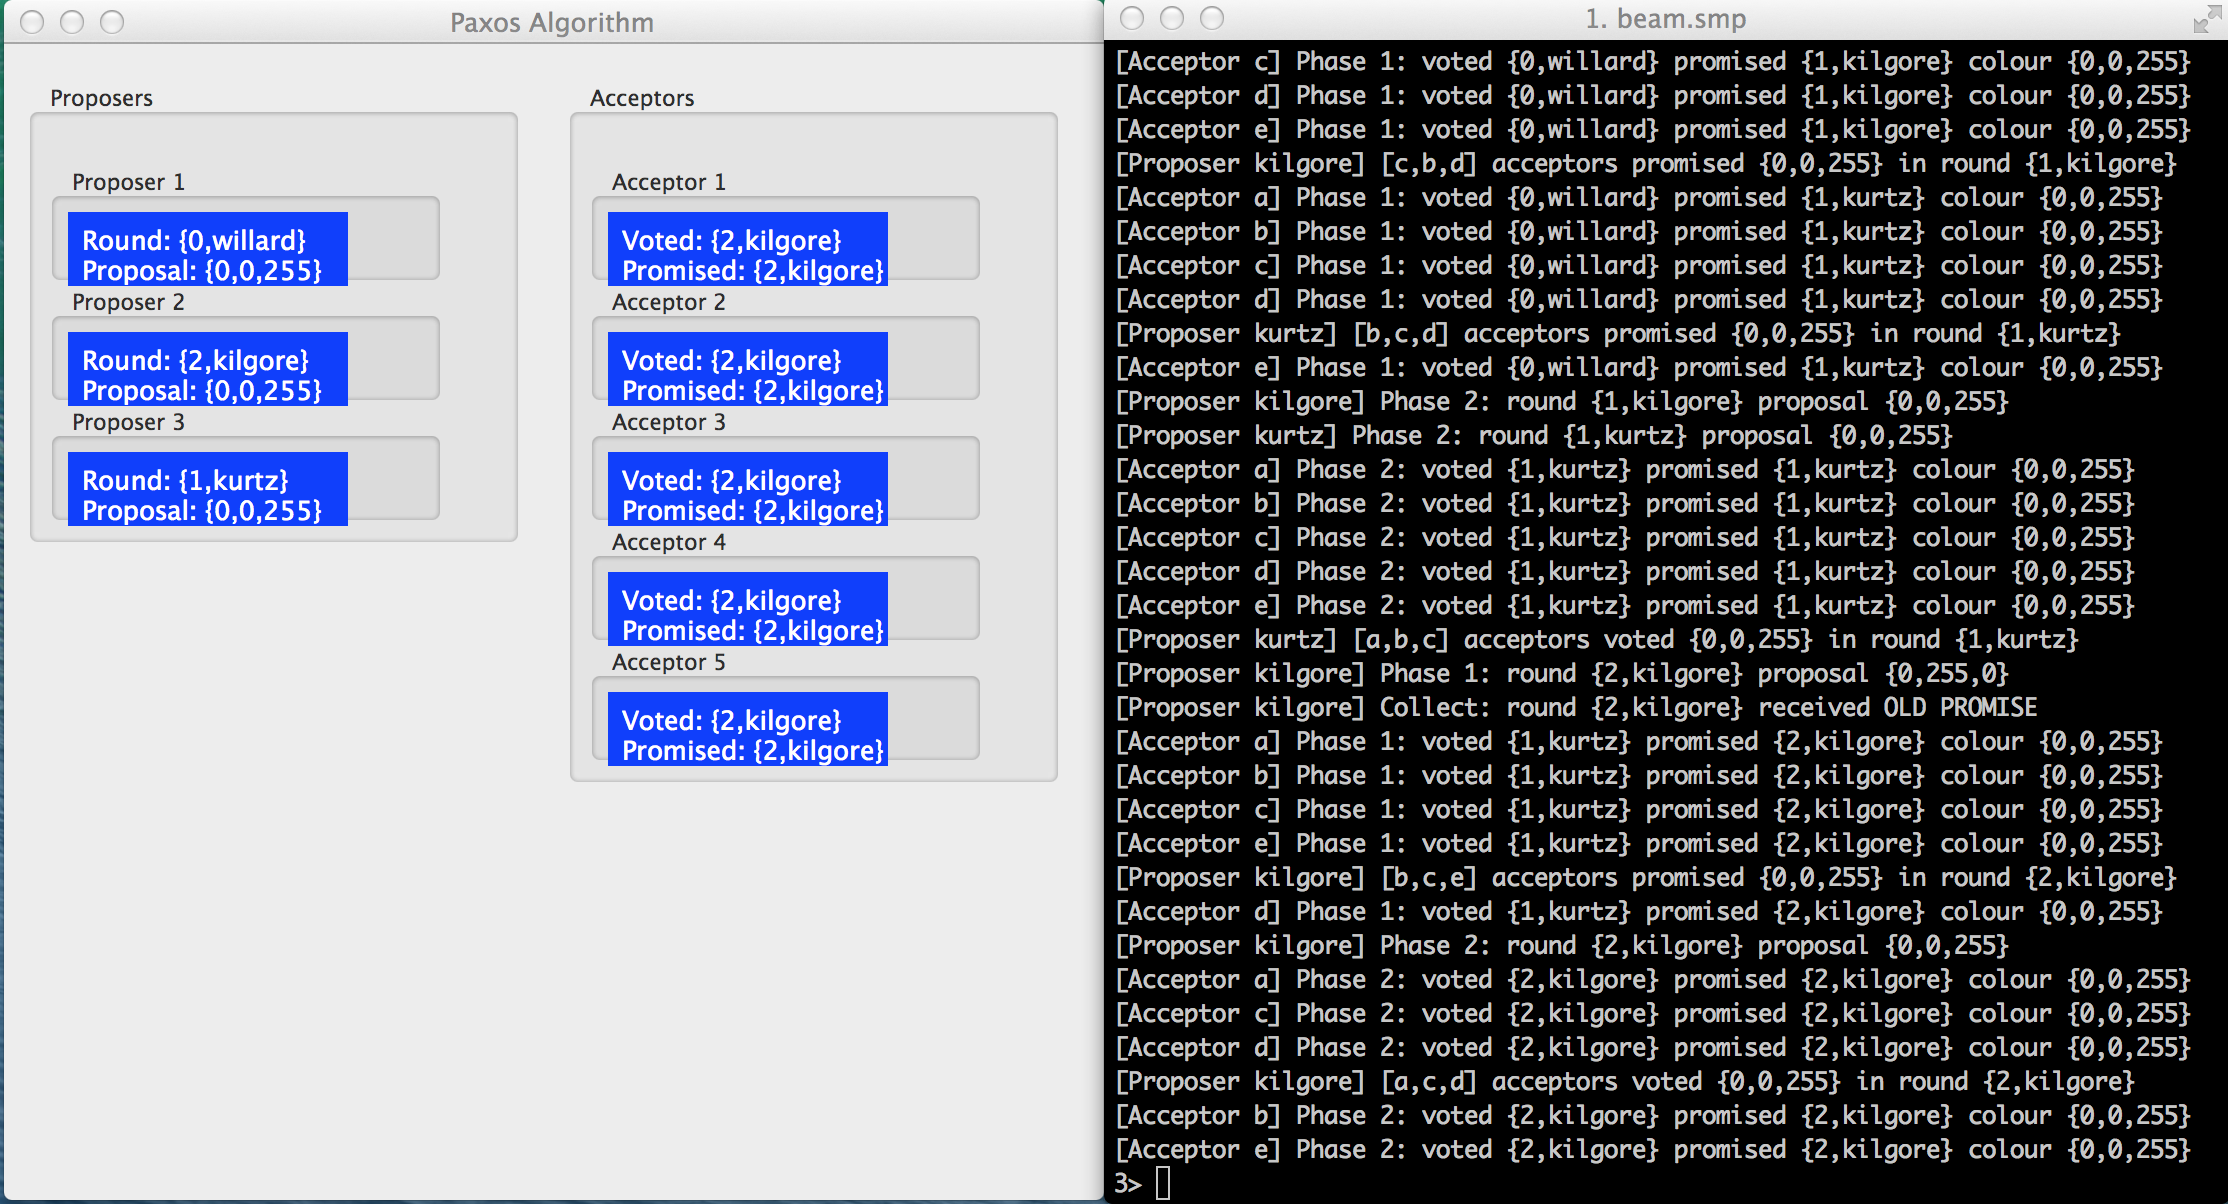
\includegraphics[scale=0.35]{images/exp4.png} \\\\

\textbf{iii)} In this experiment, we randomly drop \textit{promise} messages, and we look out for the consensus that the acceptors arrive to. Even though a promise message in round 2 is dropped, they still agree on the color blue.\\
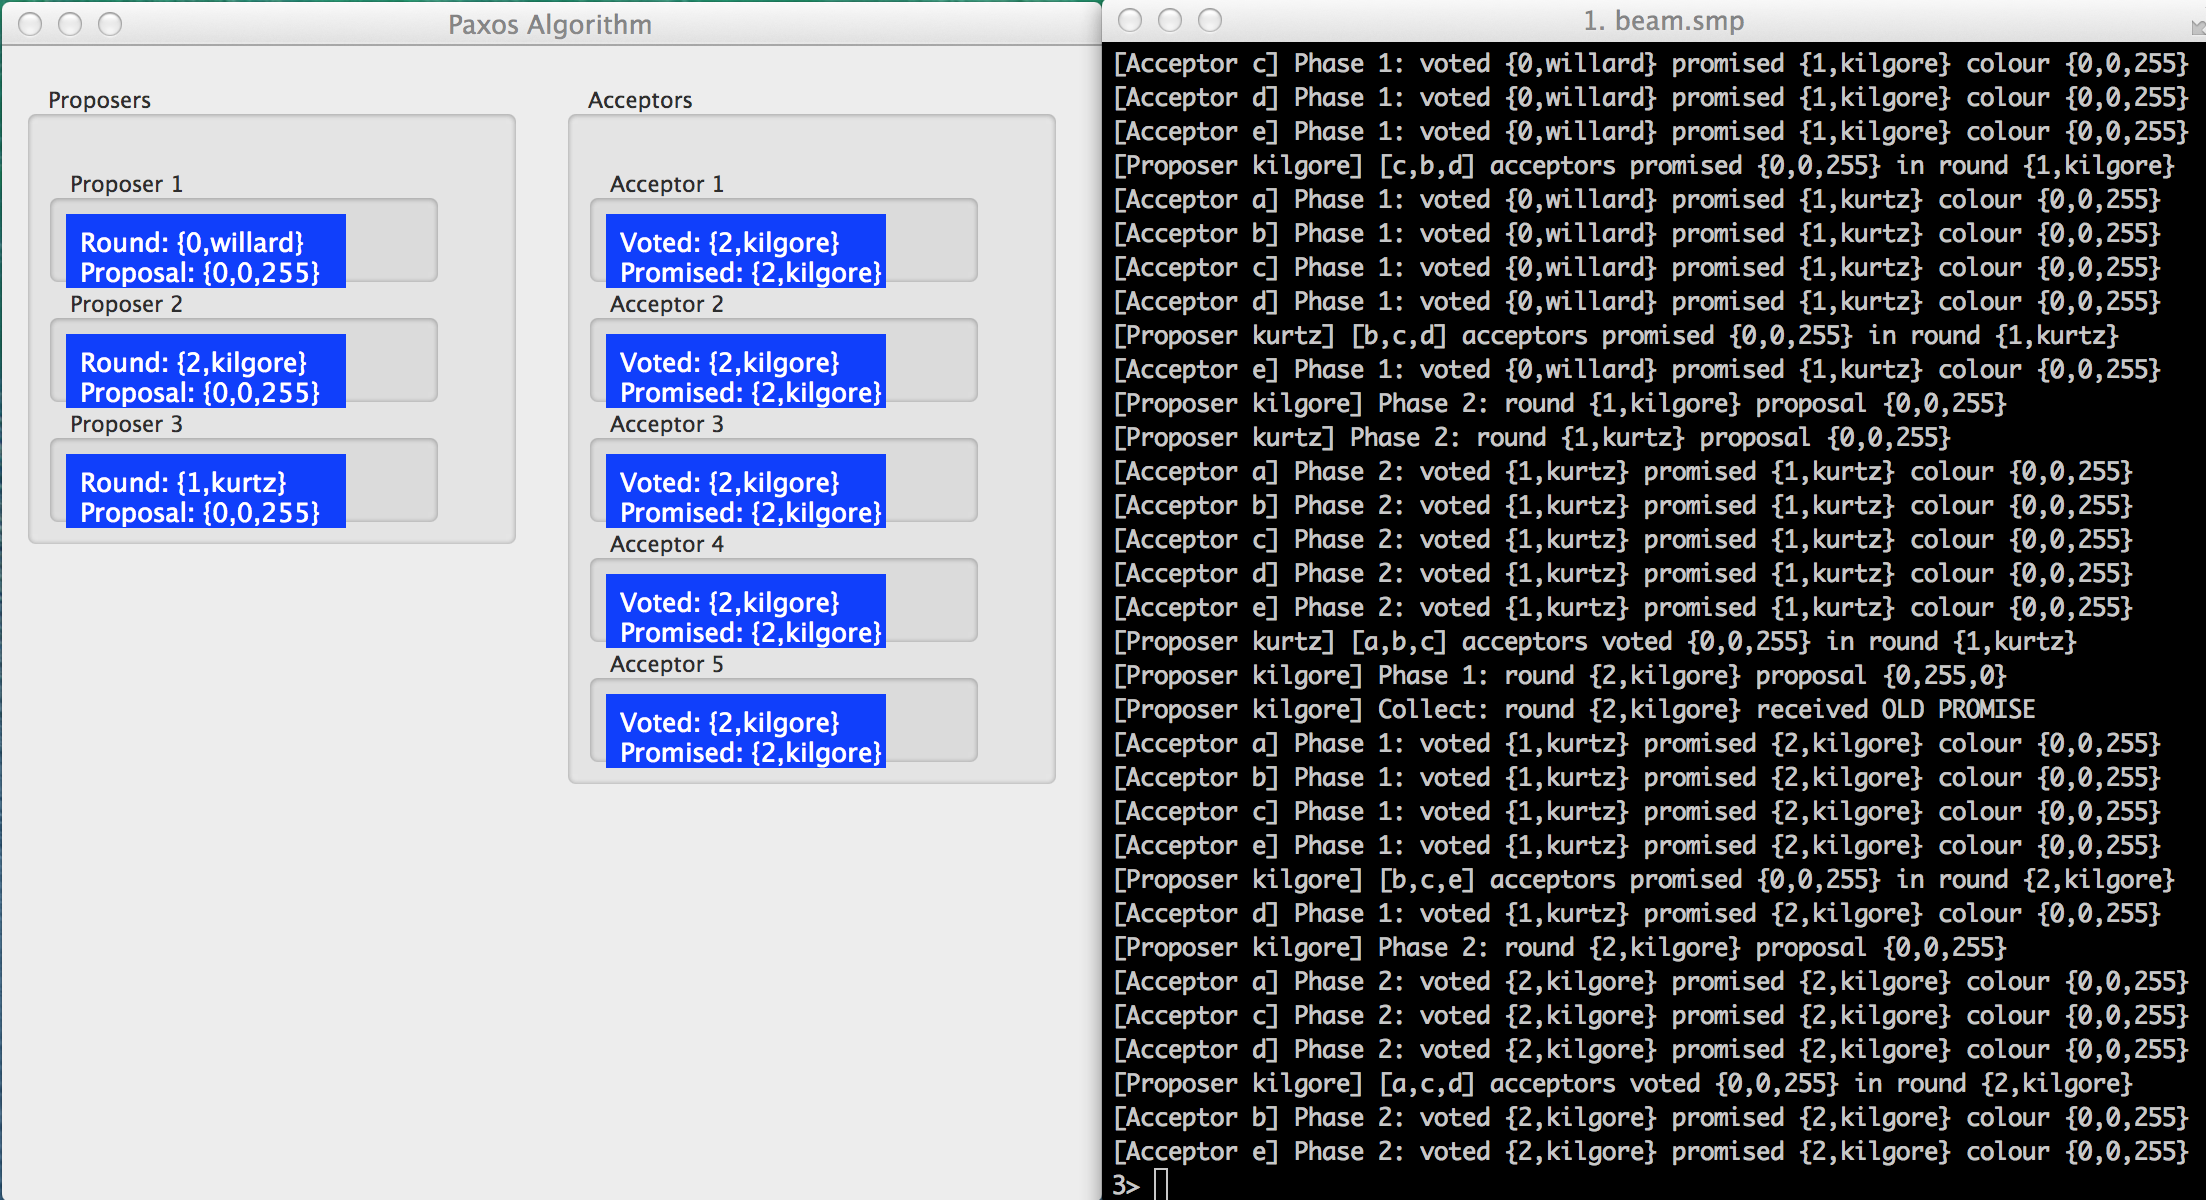
\includegraphics[scale=0.35]{images/exp5.png} \\\\
\newpage
Now, we run an experiment droping \textit{vote} messages. Again, the acceptors manage to agree on the proposed color blue, even with a \textit{vote} message dropped because the other messages still amount to the majority of acceptors.\\
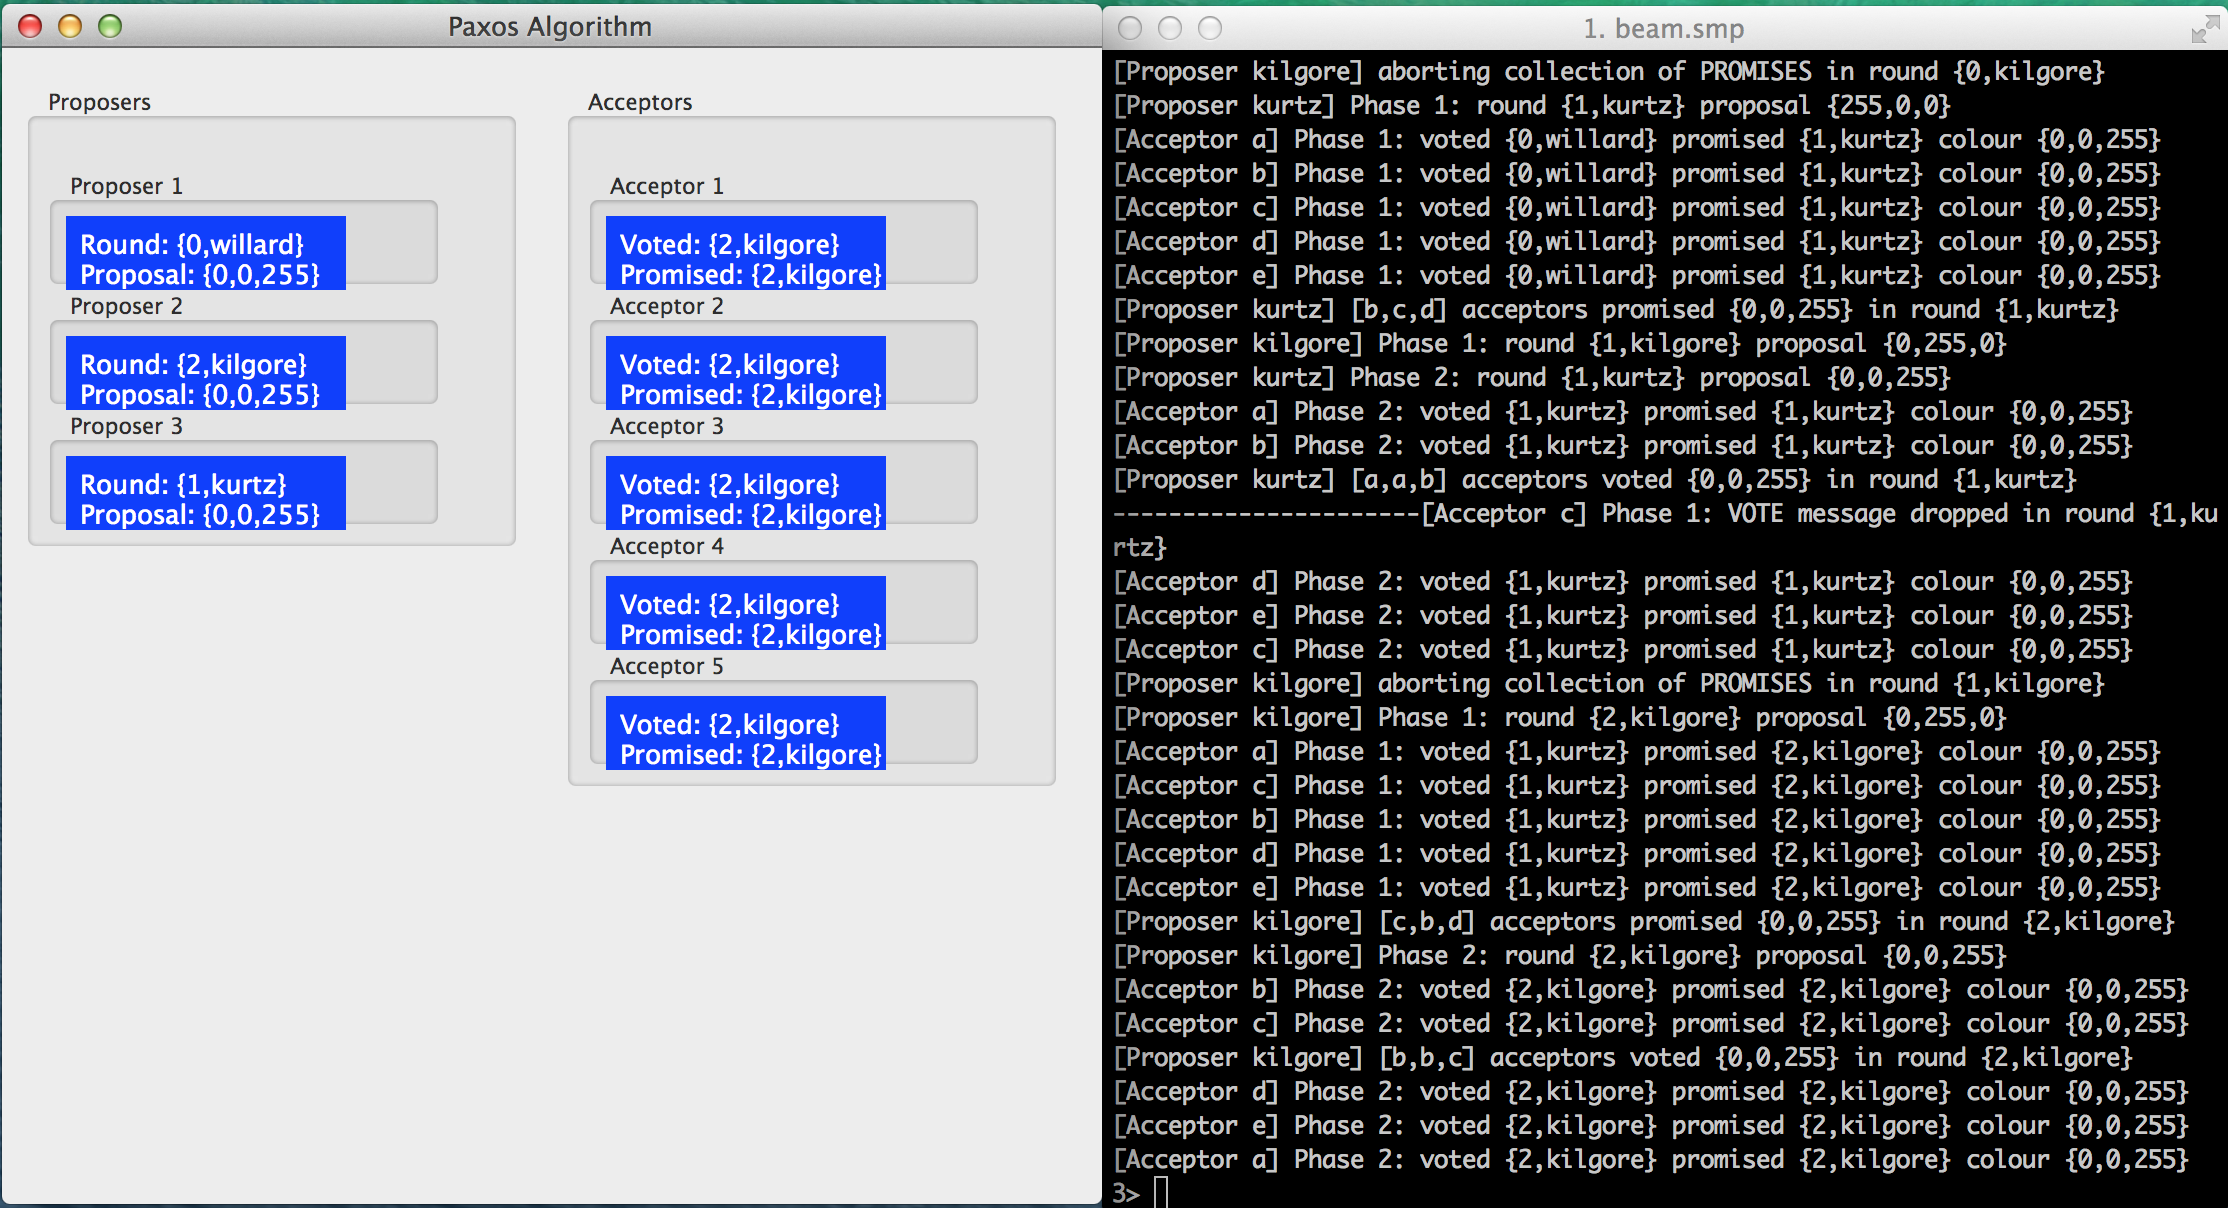
\includegraphics[scale=0.35]{images/exp6.png} \\\\
When we run the experiment dropping both \textit{promise} and \textit{vote} messages, we see that the algorithm still terminates successfully due to the fact that the majority of acceptors whose messages were not dropped agreed.\\
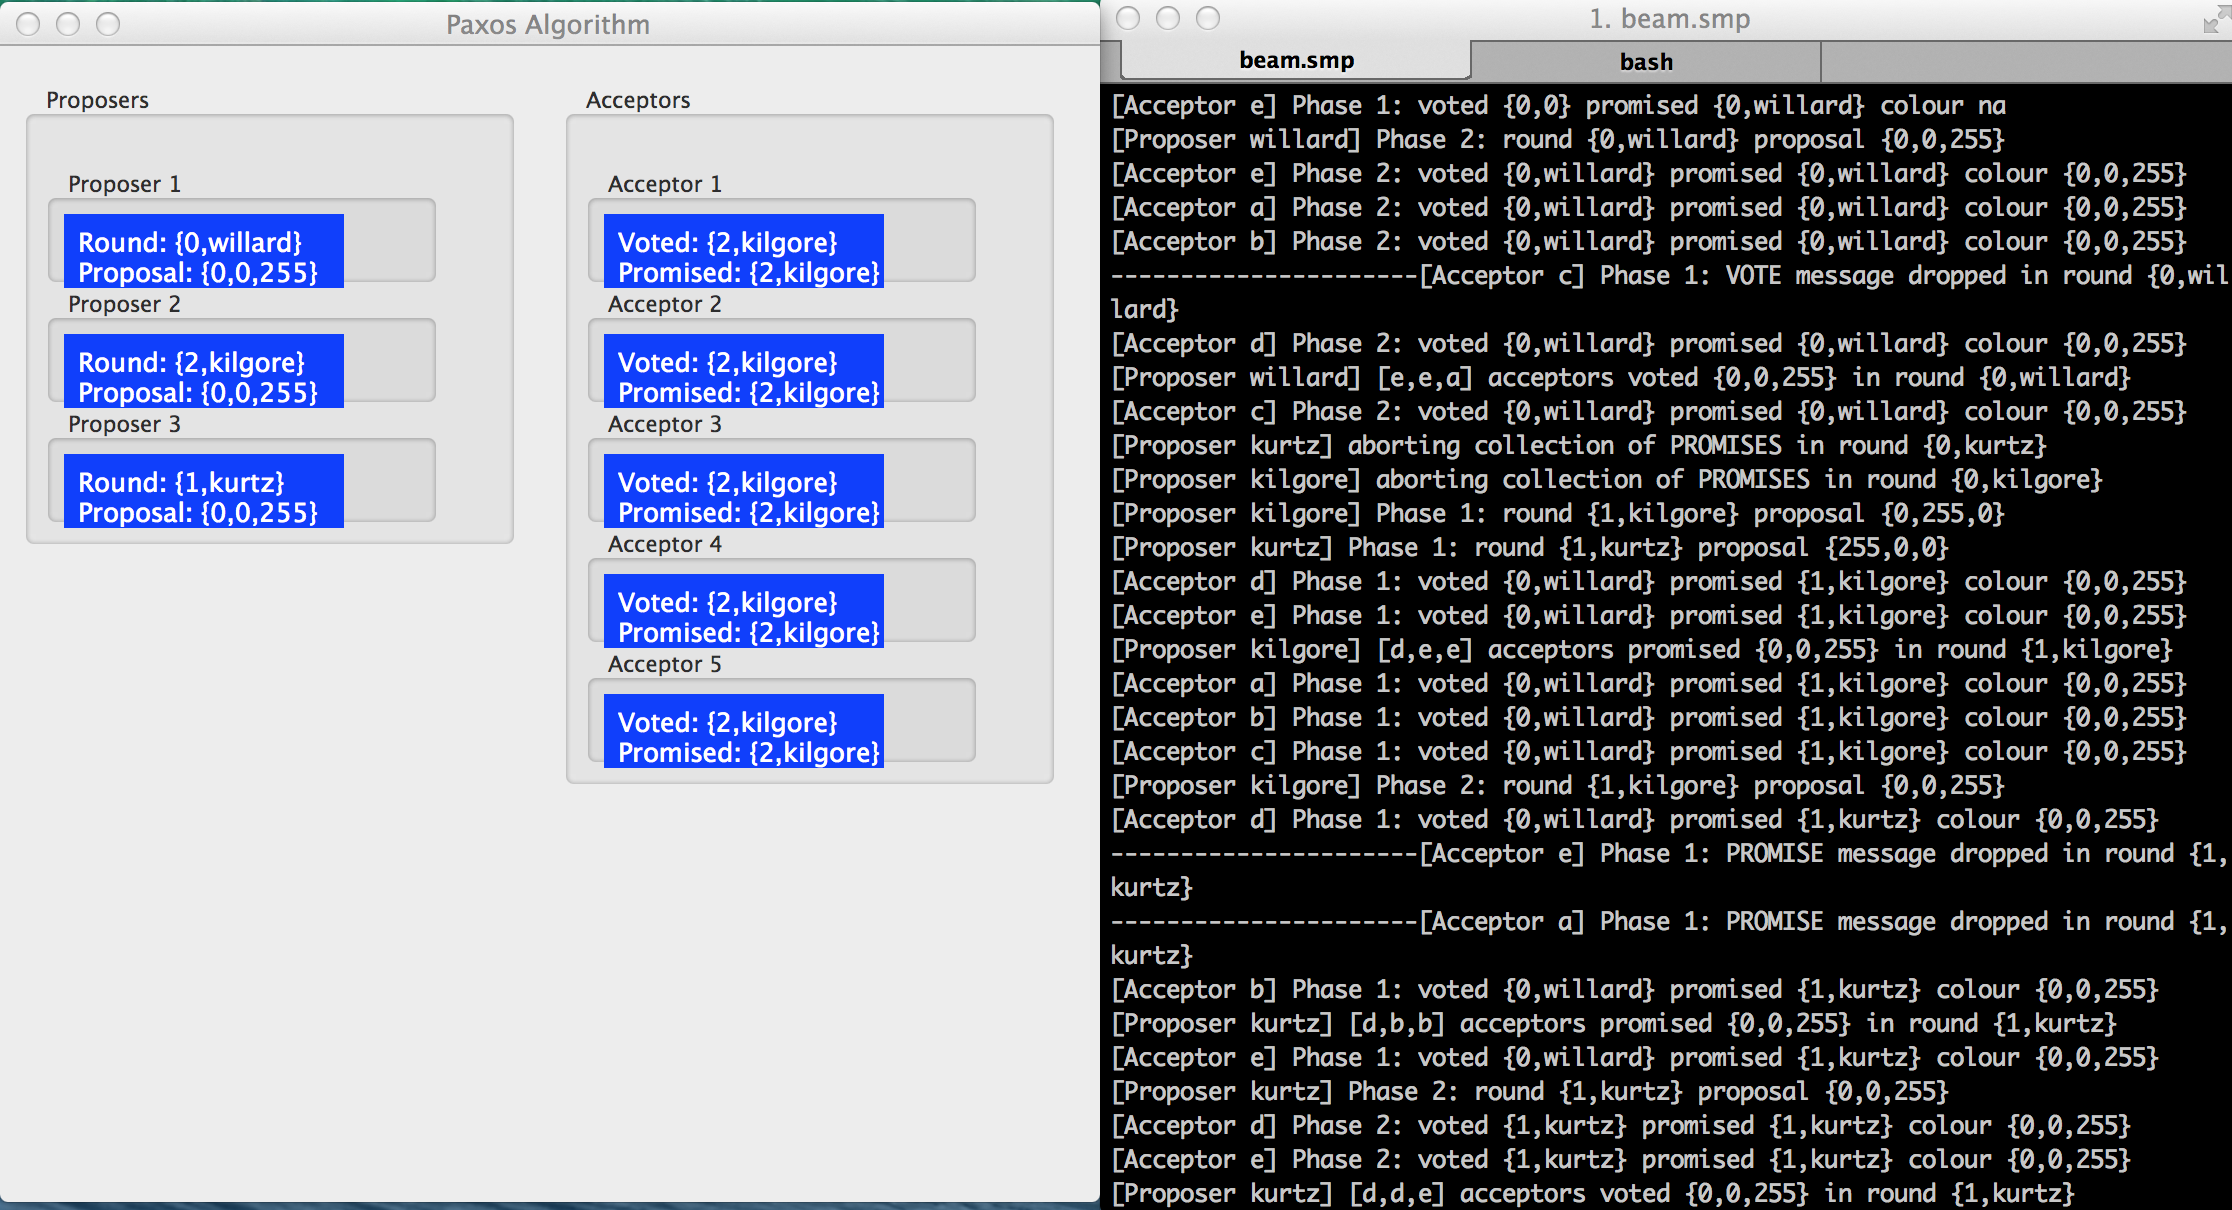
\includegraphics[scale=0.35]{images/exp7.png} \\\\
\newpage
We also run the experiment by dropping more than one \textit{promise} and \textit{vote} messages in a total of 10 messages. Here is the result of dropping one message in 5. The algorithm still terminates and the acceptors reach the consensus.\\
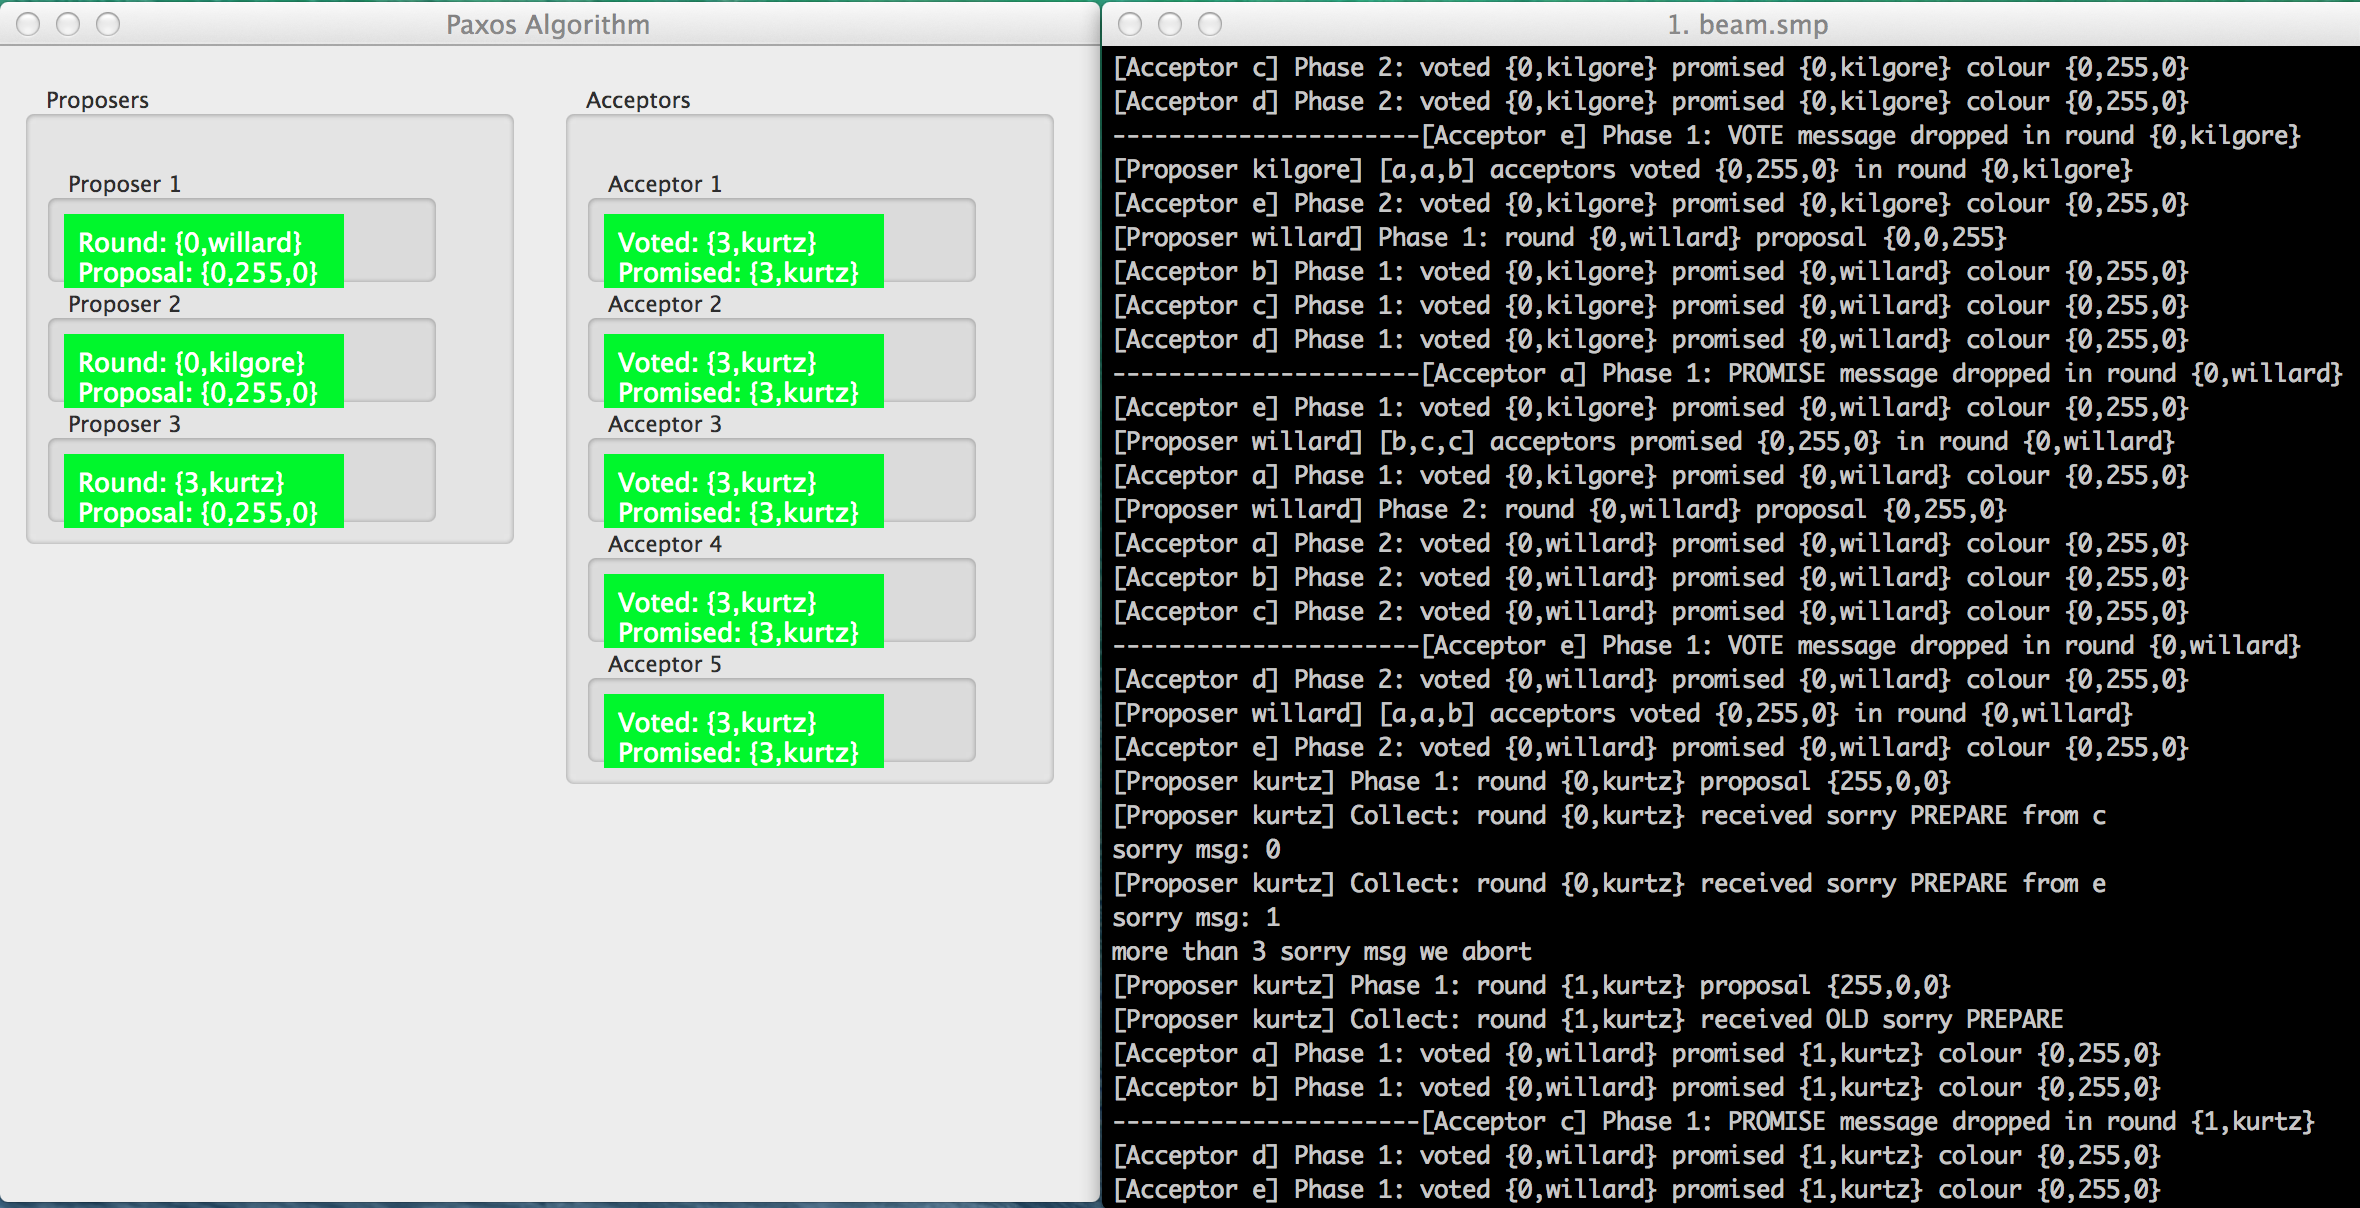
\includegraphics[scale=0.35]{images/exp7-drop5.png} \\\\
We ran more experiments by dropping one message in 3:\\
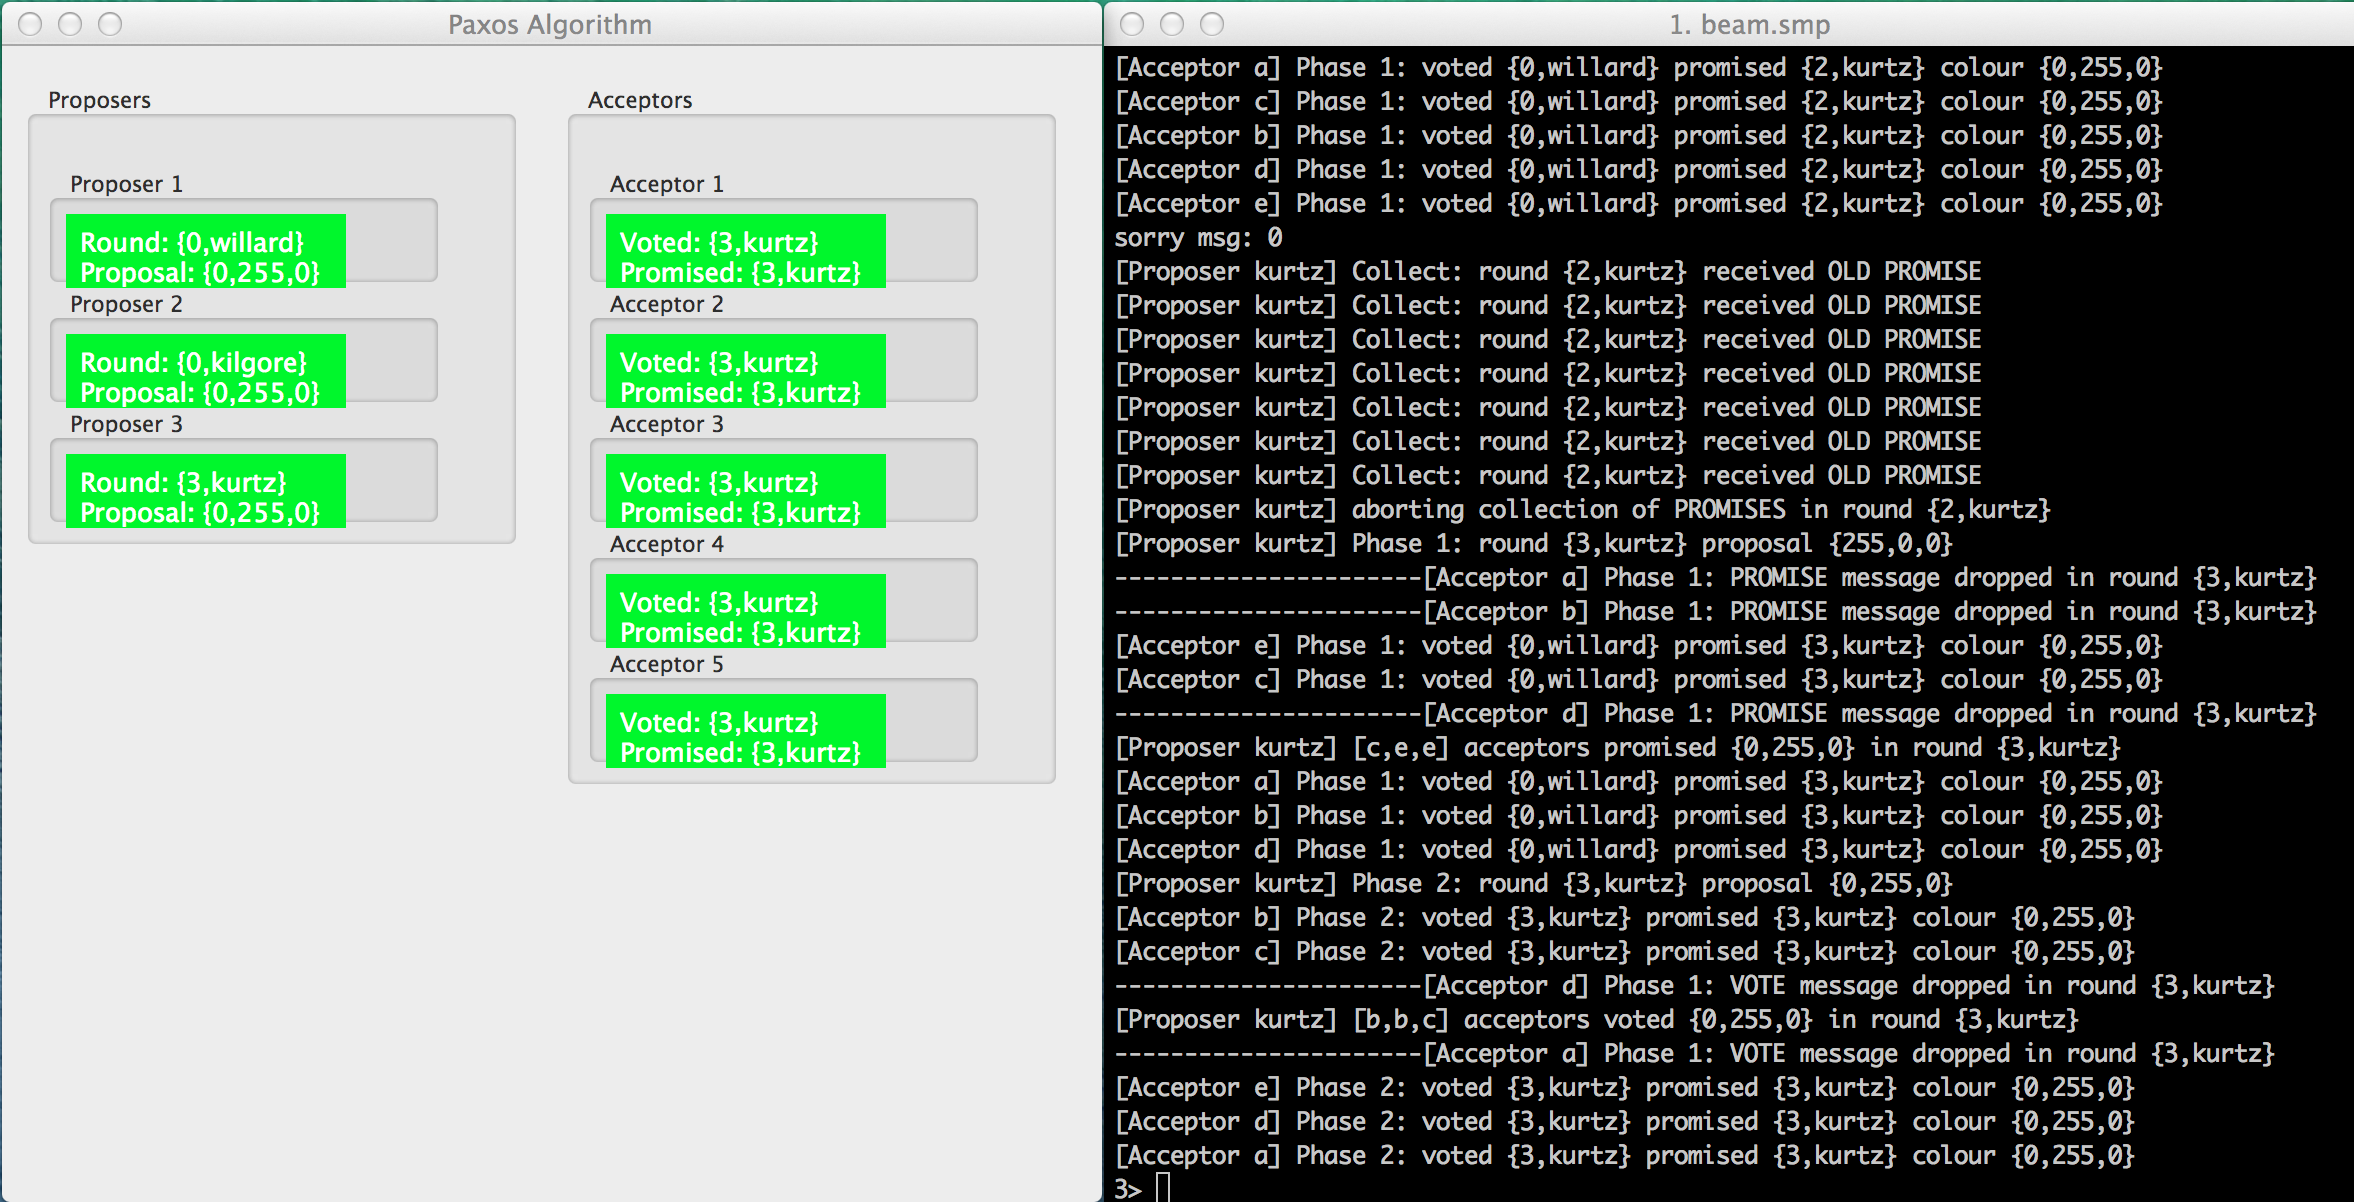
\includegraphics[scale=0.35]{images/exp7-drop3.png} \\\\
\newpage
And one message in 1:\\
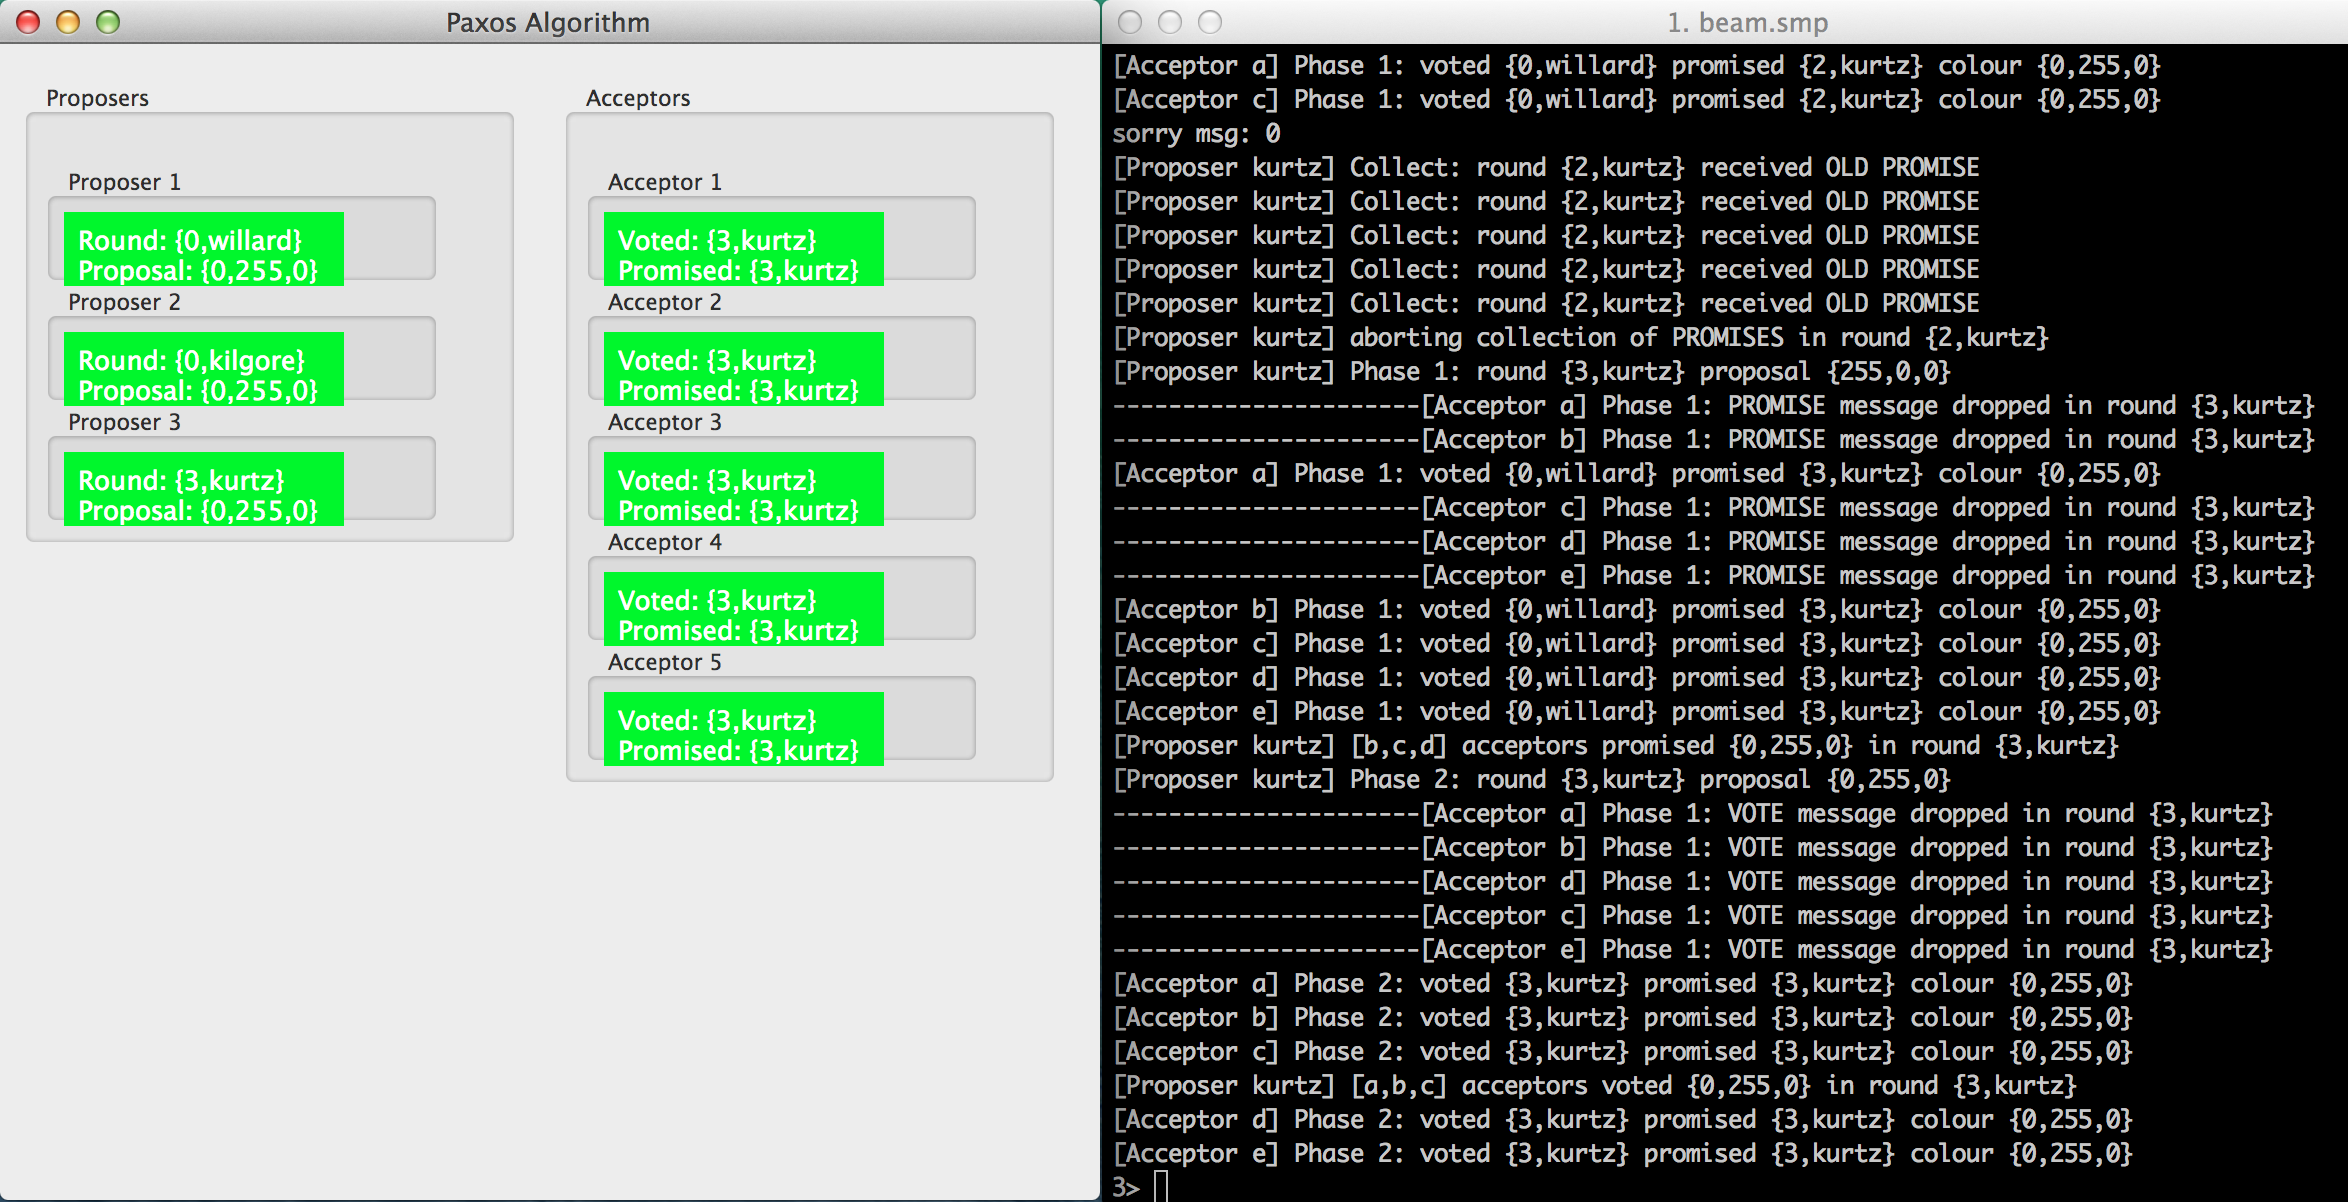
\includegraphics[scale=0.35]{images/exp7-drop1.png} \\\\
And even though more and more messages are dropped an agreement is eventually met. However if we add the line: \textit{-define(drop, 0).} then the algorithm does not terminate.\\
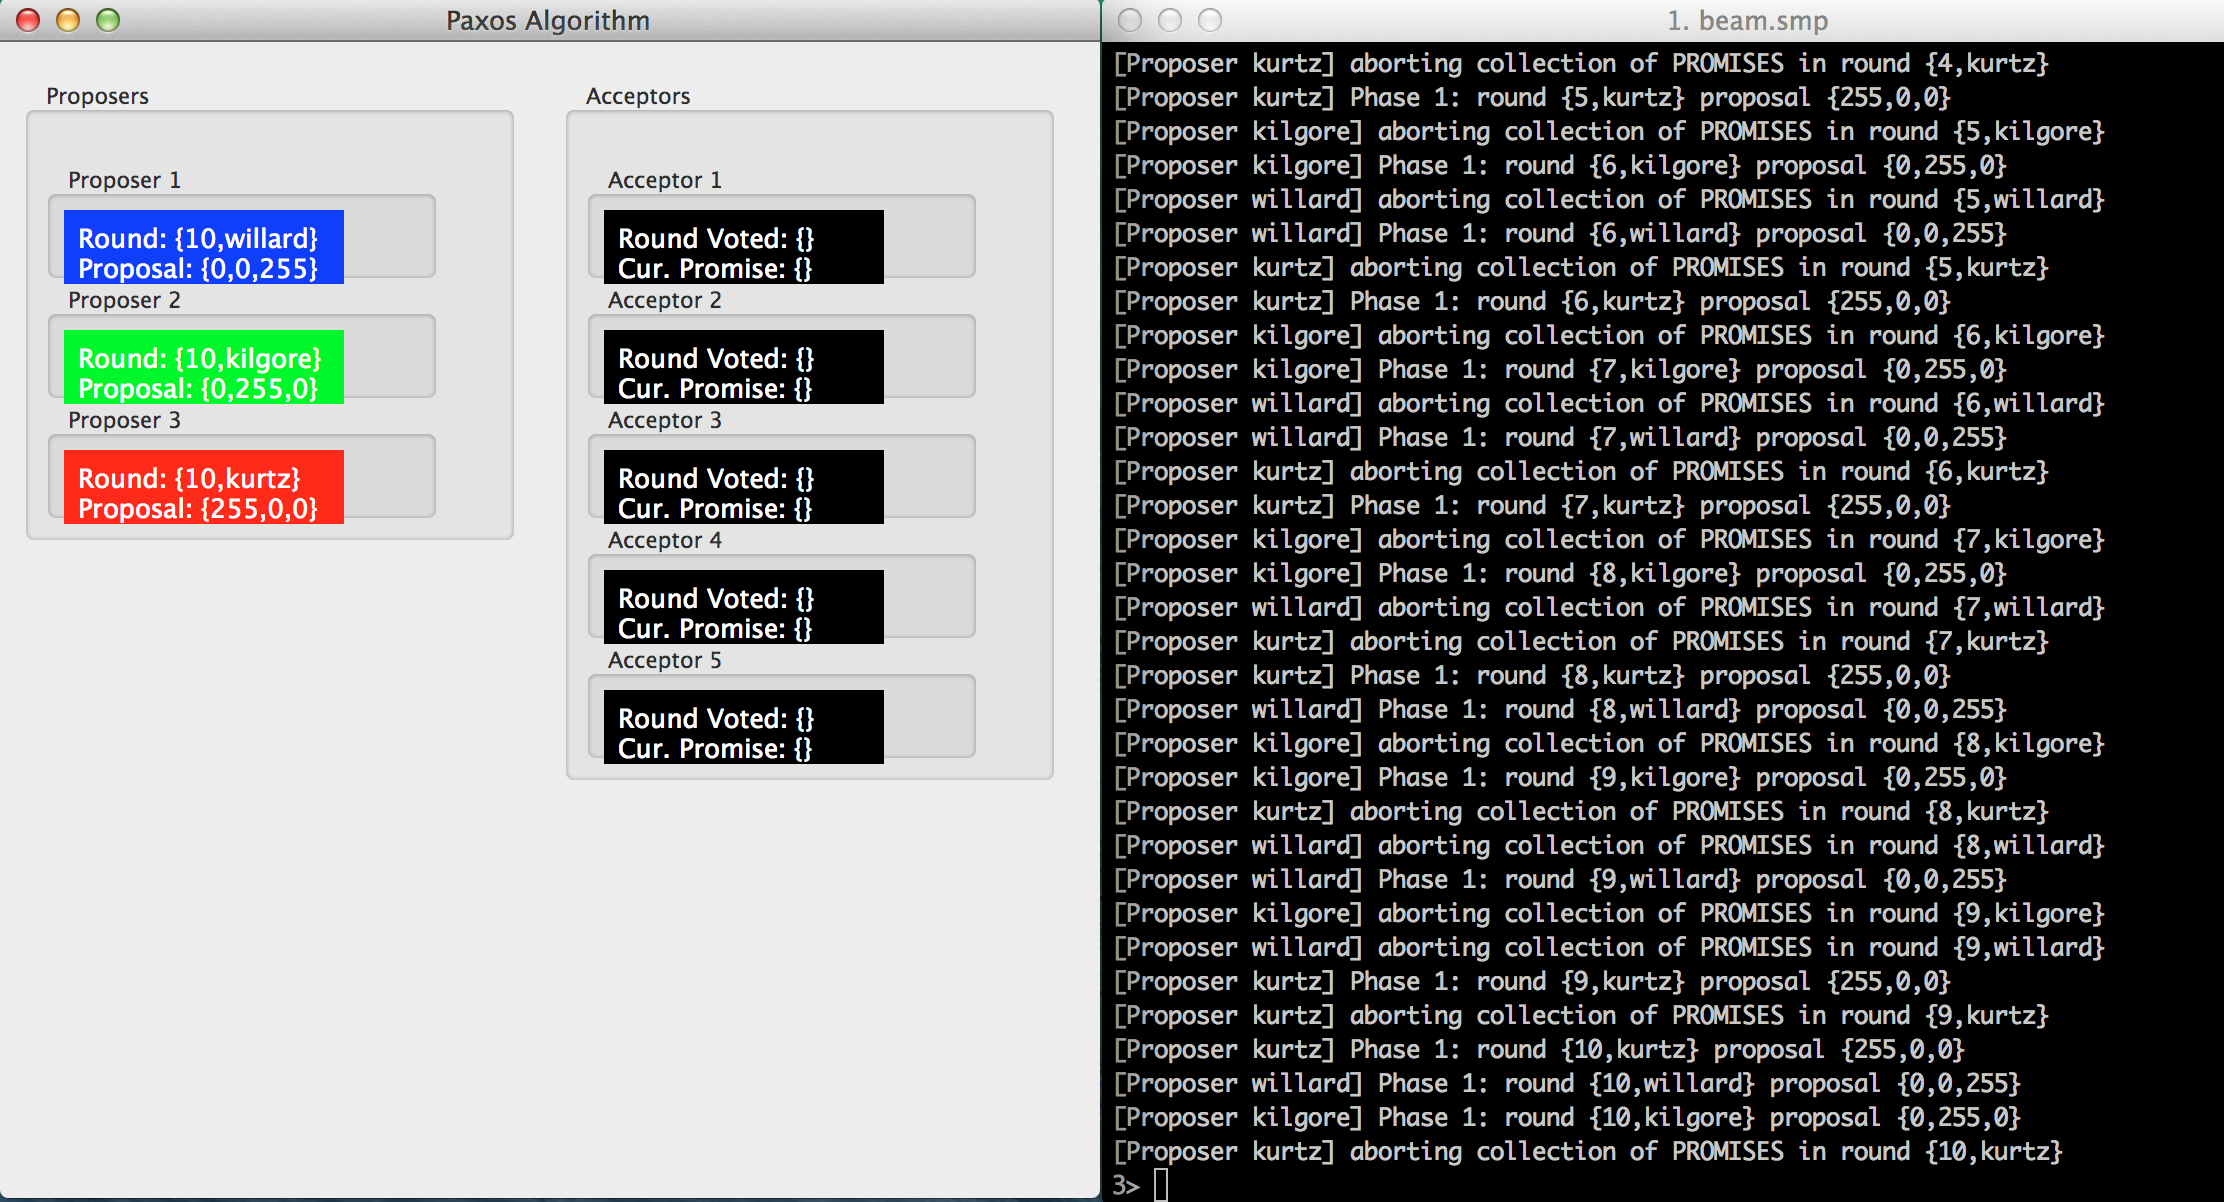
\includegraphics[scale=0.35]{images/exp7-drop0.png} \\\\
\newpage
\textbf{iv)} We increase the number of acceptors to 10 and the number or proposers to 6. The acceptors still get to a consensuns in round 3 on color \textit{purple}.\\
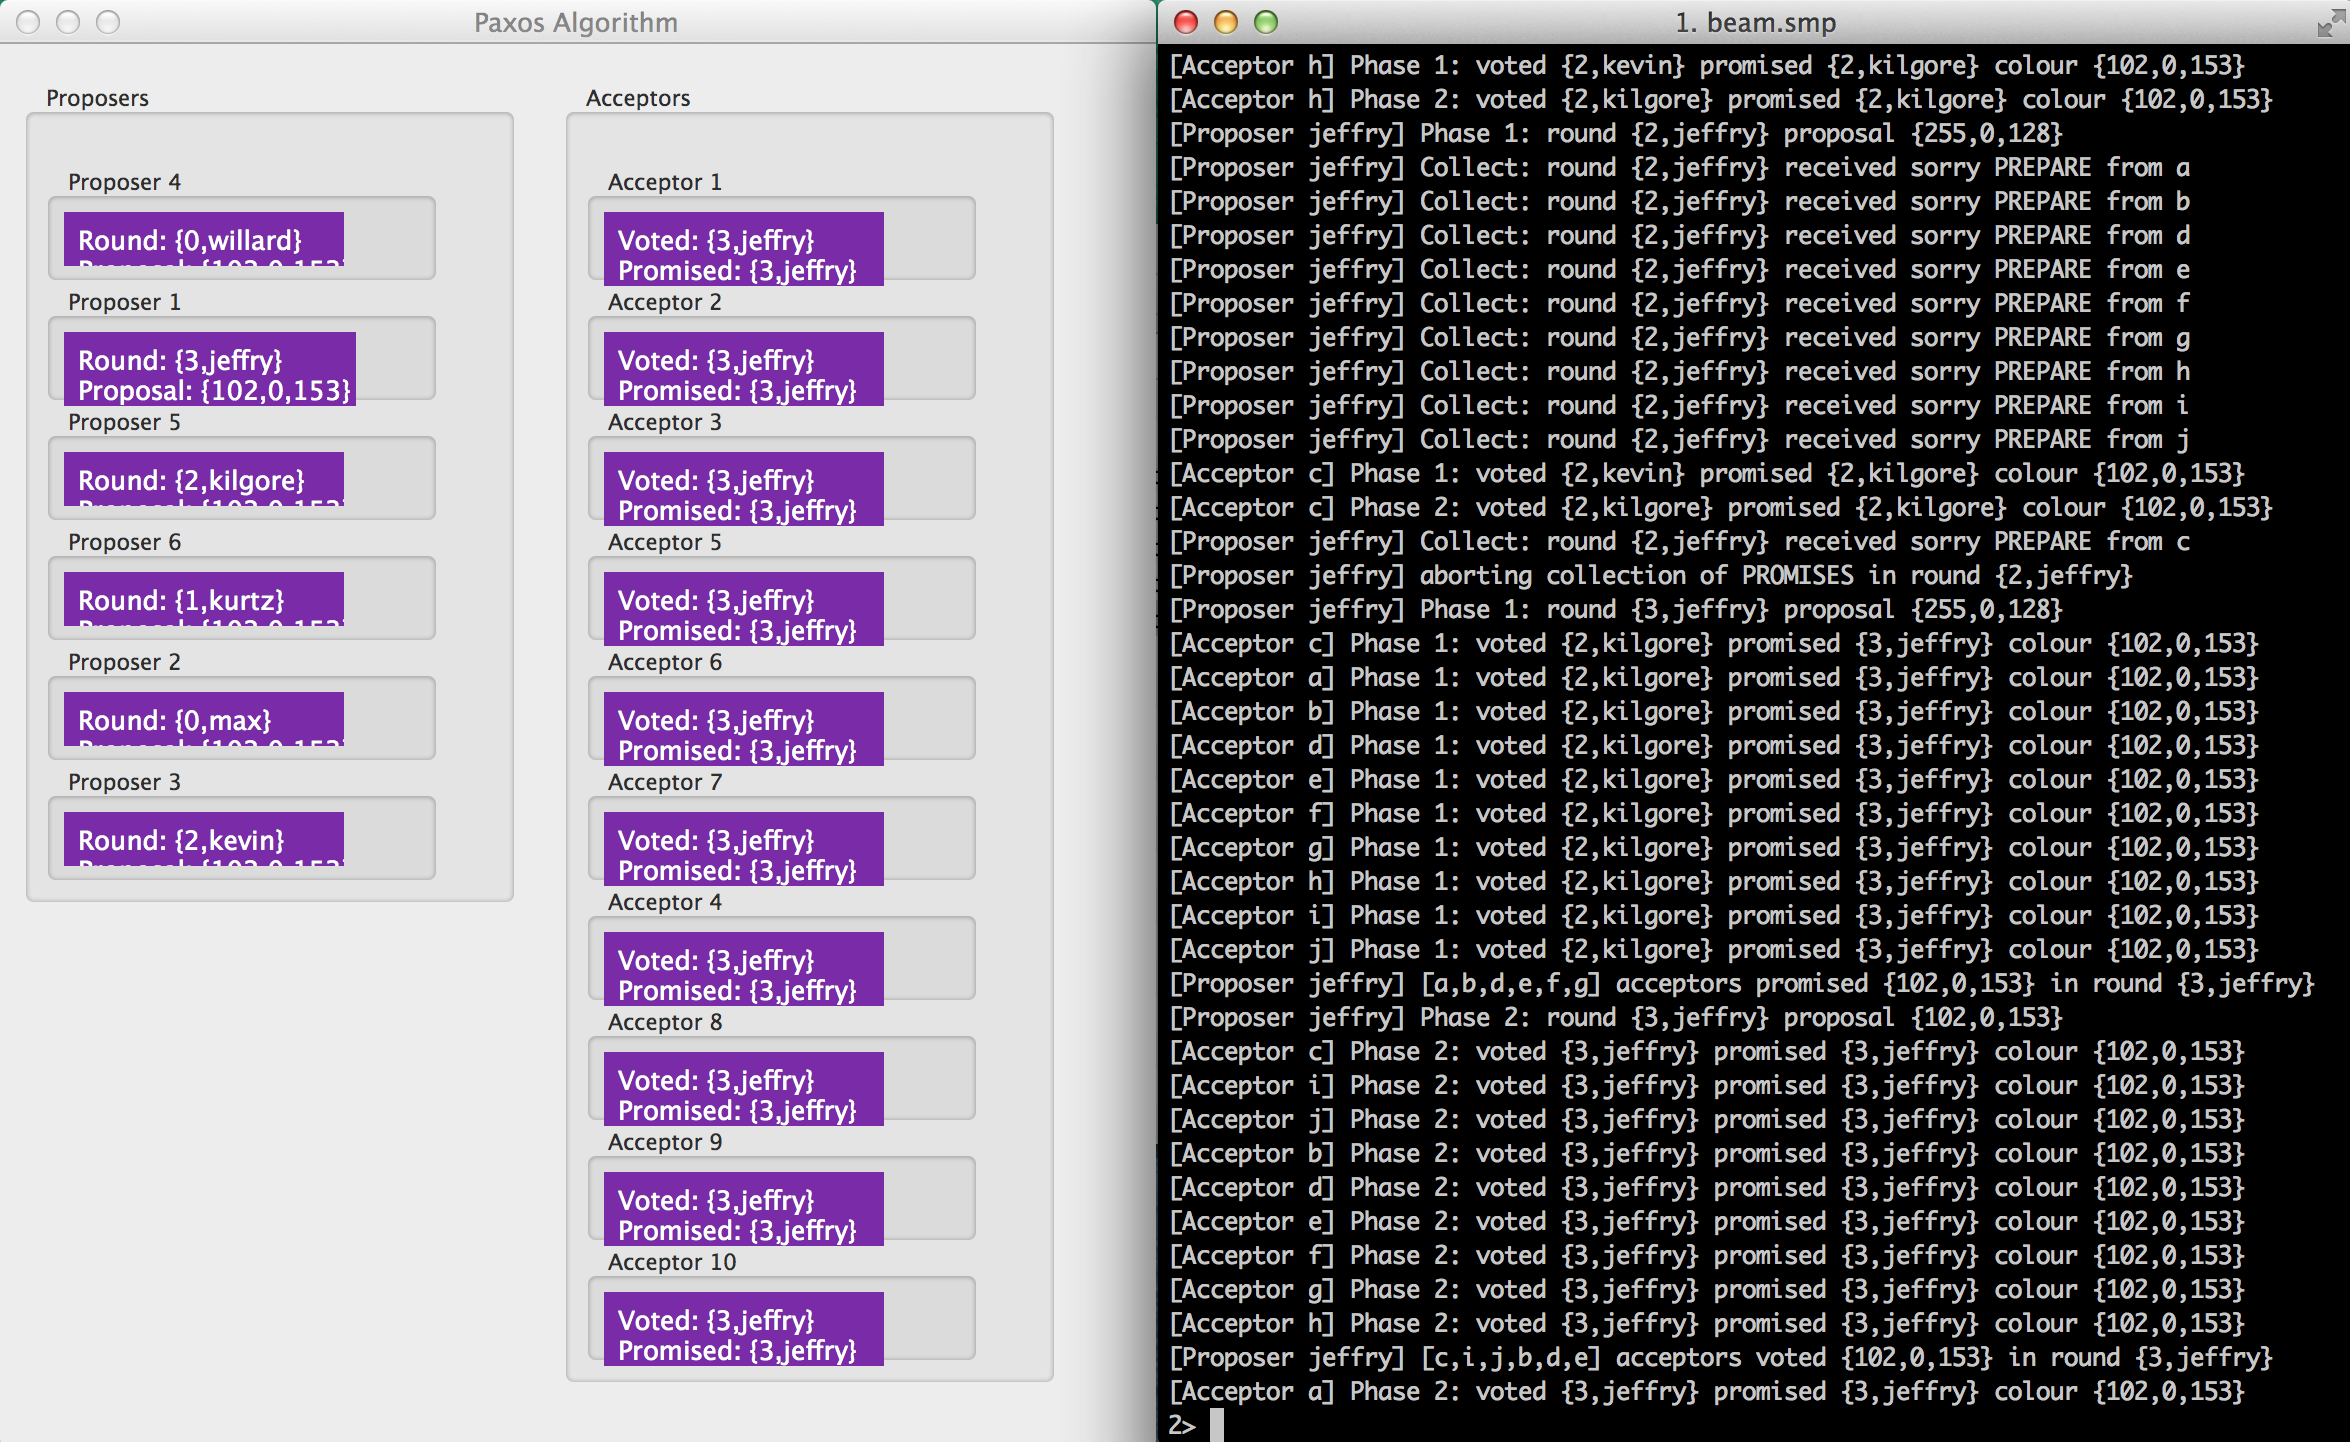
\includegraphics[scale=0.30]{images/exp8.png} \\\\

\textbf{v)} In this experiment we changed the modules to adjust them such that we can run the proposers in one machine and the acceptors in a different one and as they communicate they reach an agreement on the color \textit{blue} in round 2.\\
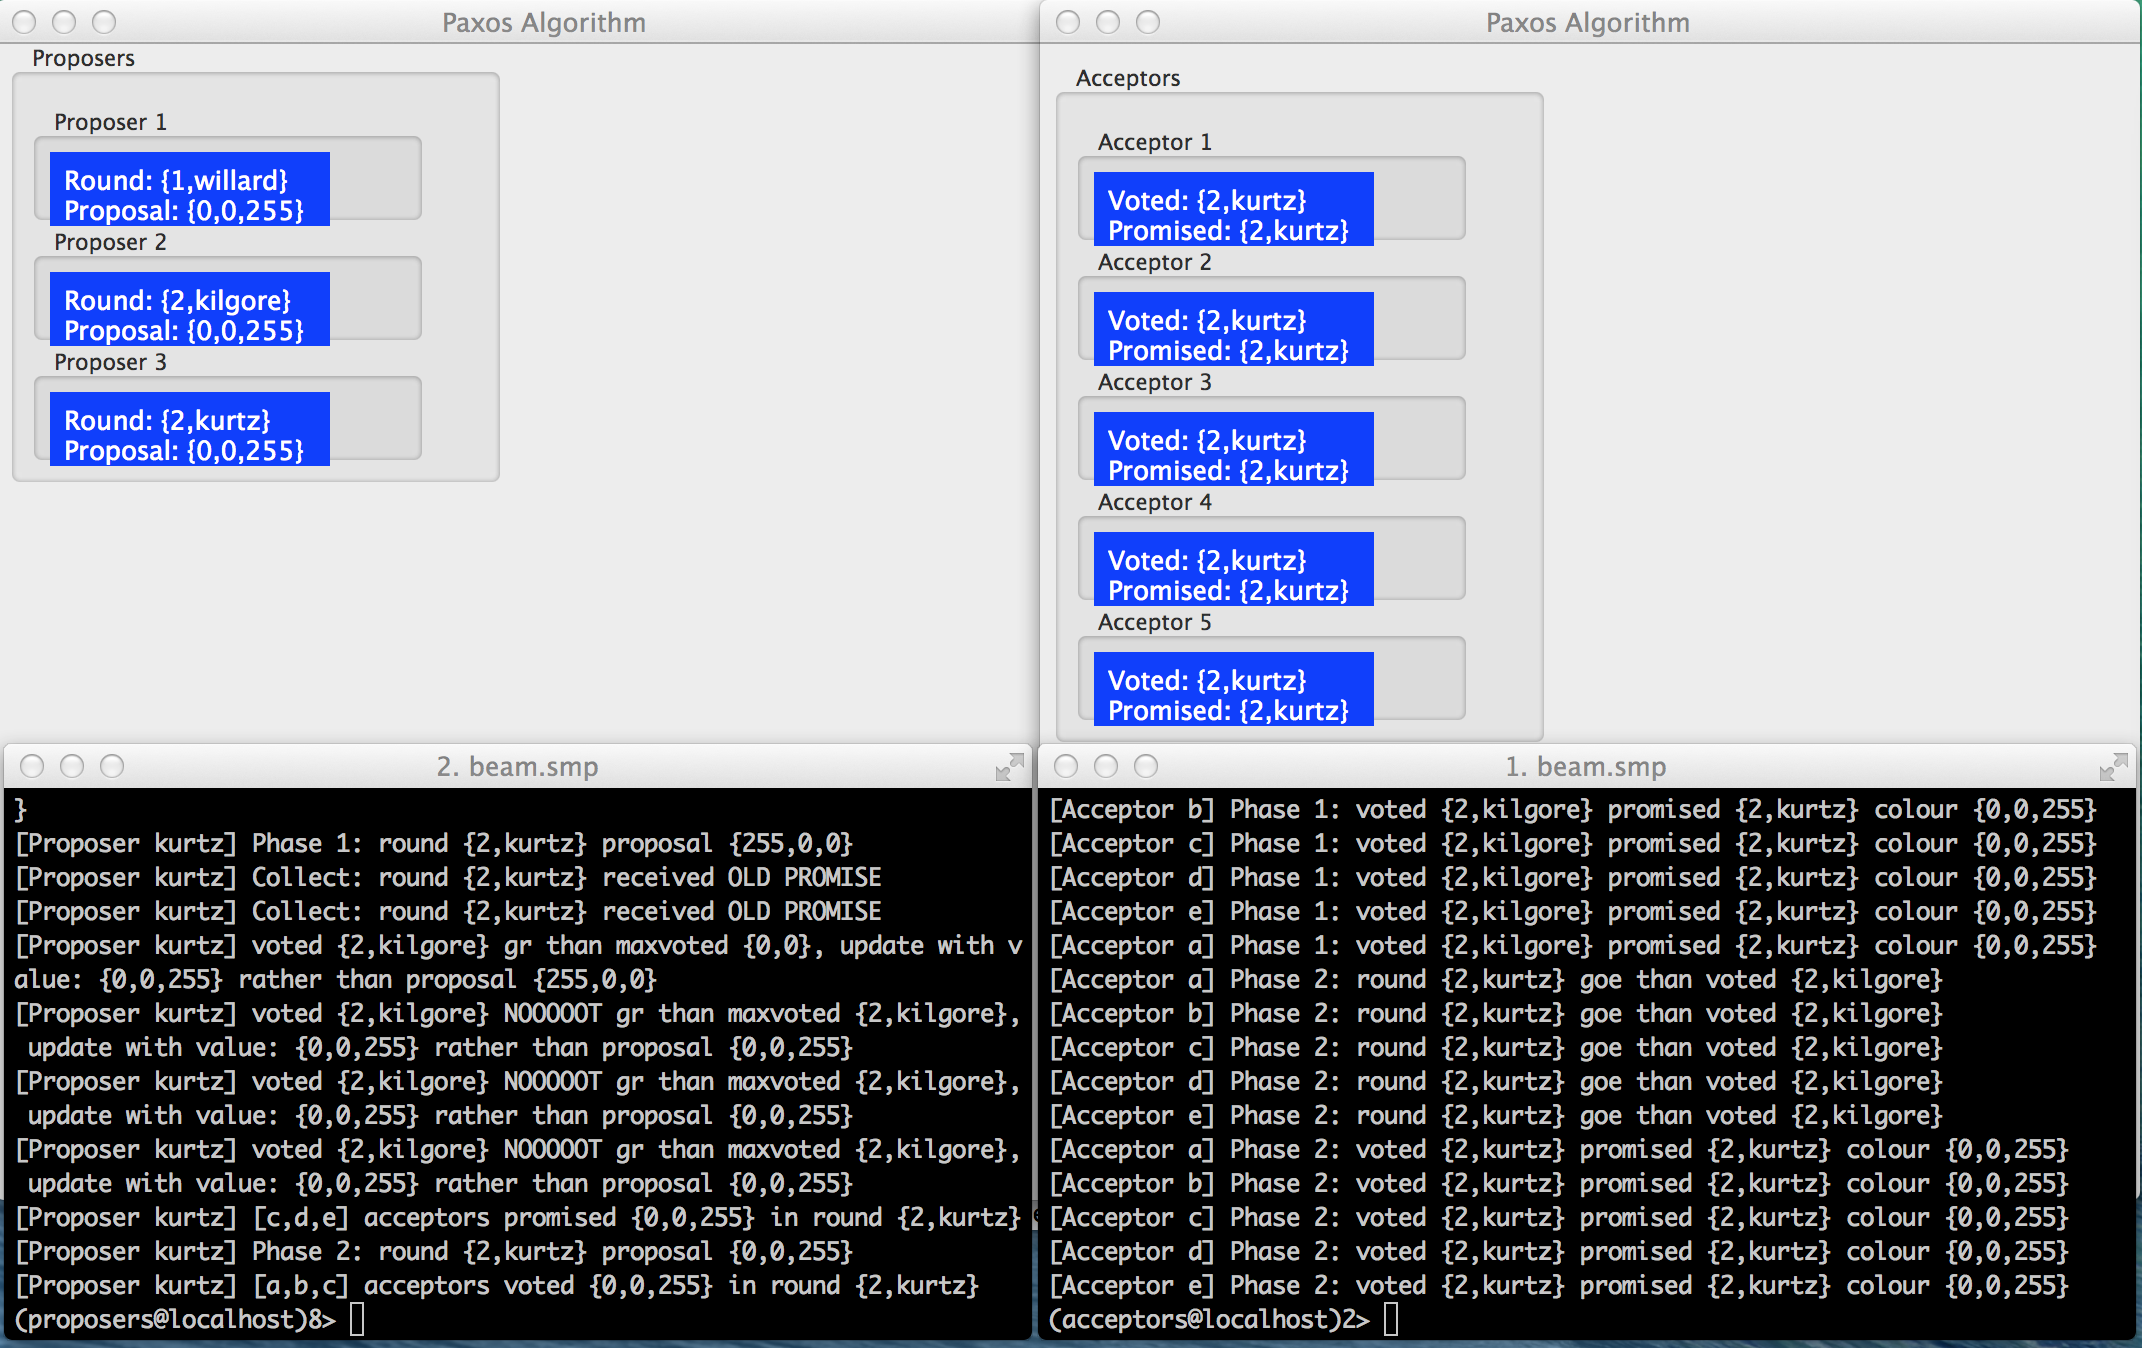
\includegraphics[scale=0.30]{images/exp9.png} \\\\
\newpage
\textbf{Fault Tollerance}
In order to test the fault tollerance we added the \textit{crash} function in the paxy module and while running the experiment, we crashed one of the acceptors. Analyzing the trace we see that the acceptor starts again and continues to participate and the algorithm terminates. We ran the experiment both on the same machine and on separate machines for the proposers and acceptors.\\
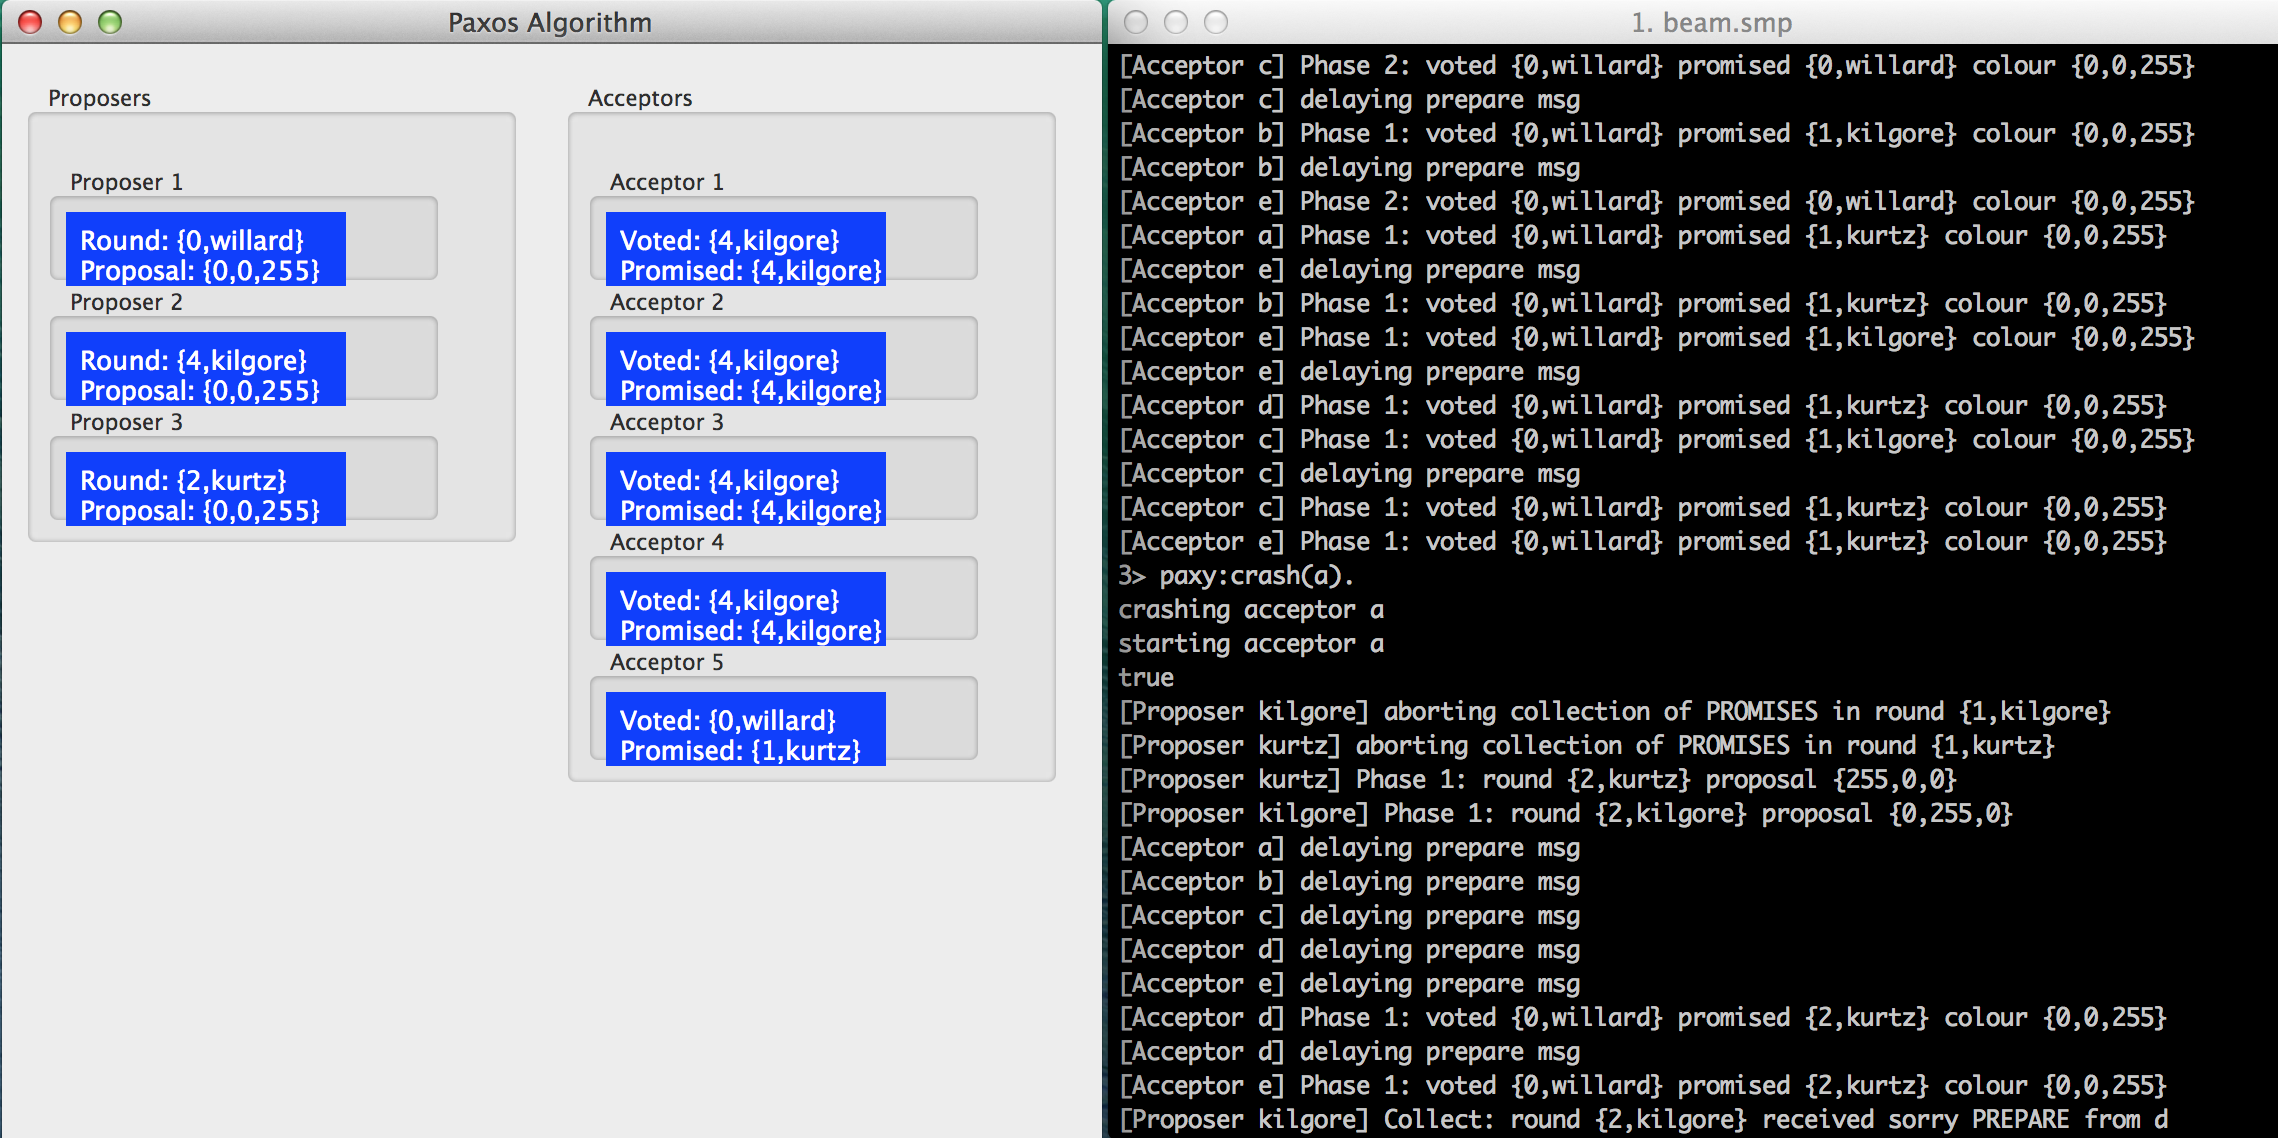
\includegraphics[scale=0.35]{images/exp10.png} \\\\
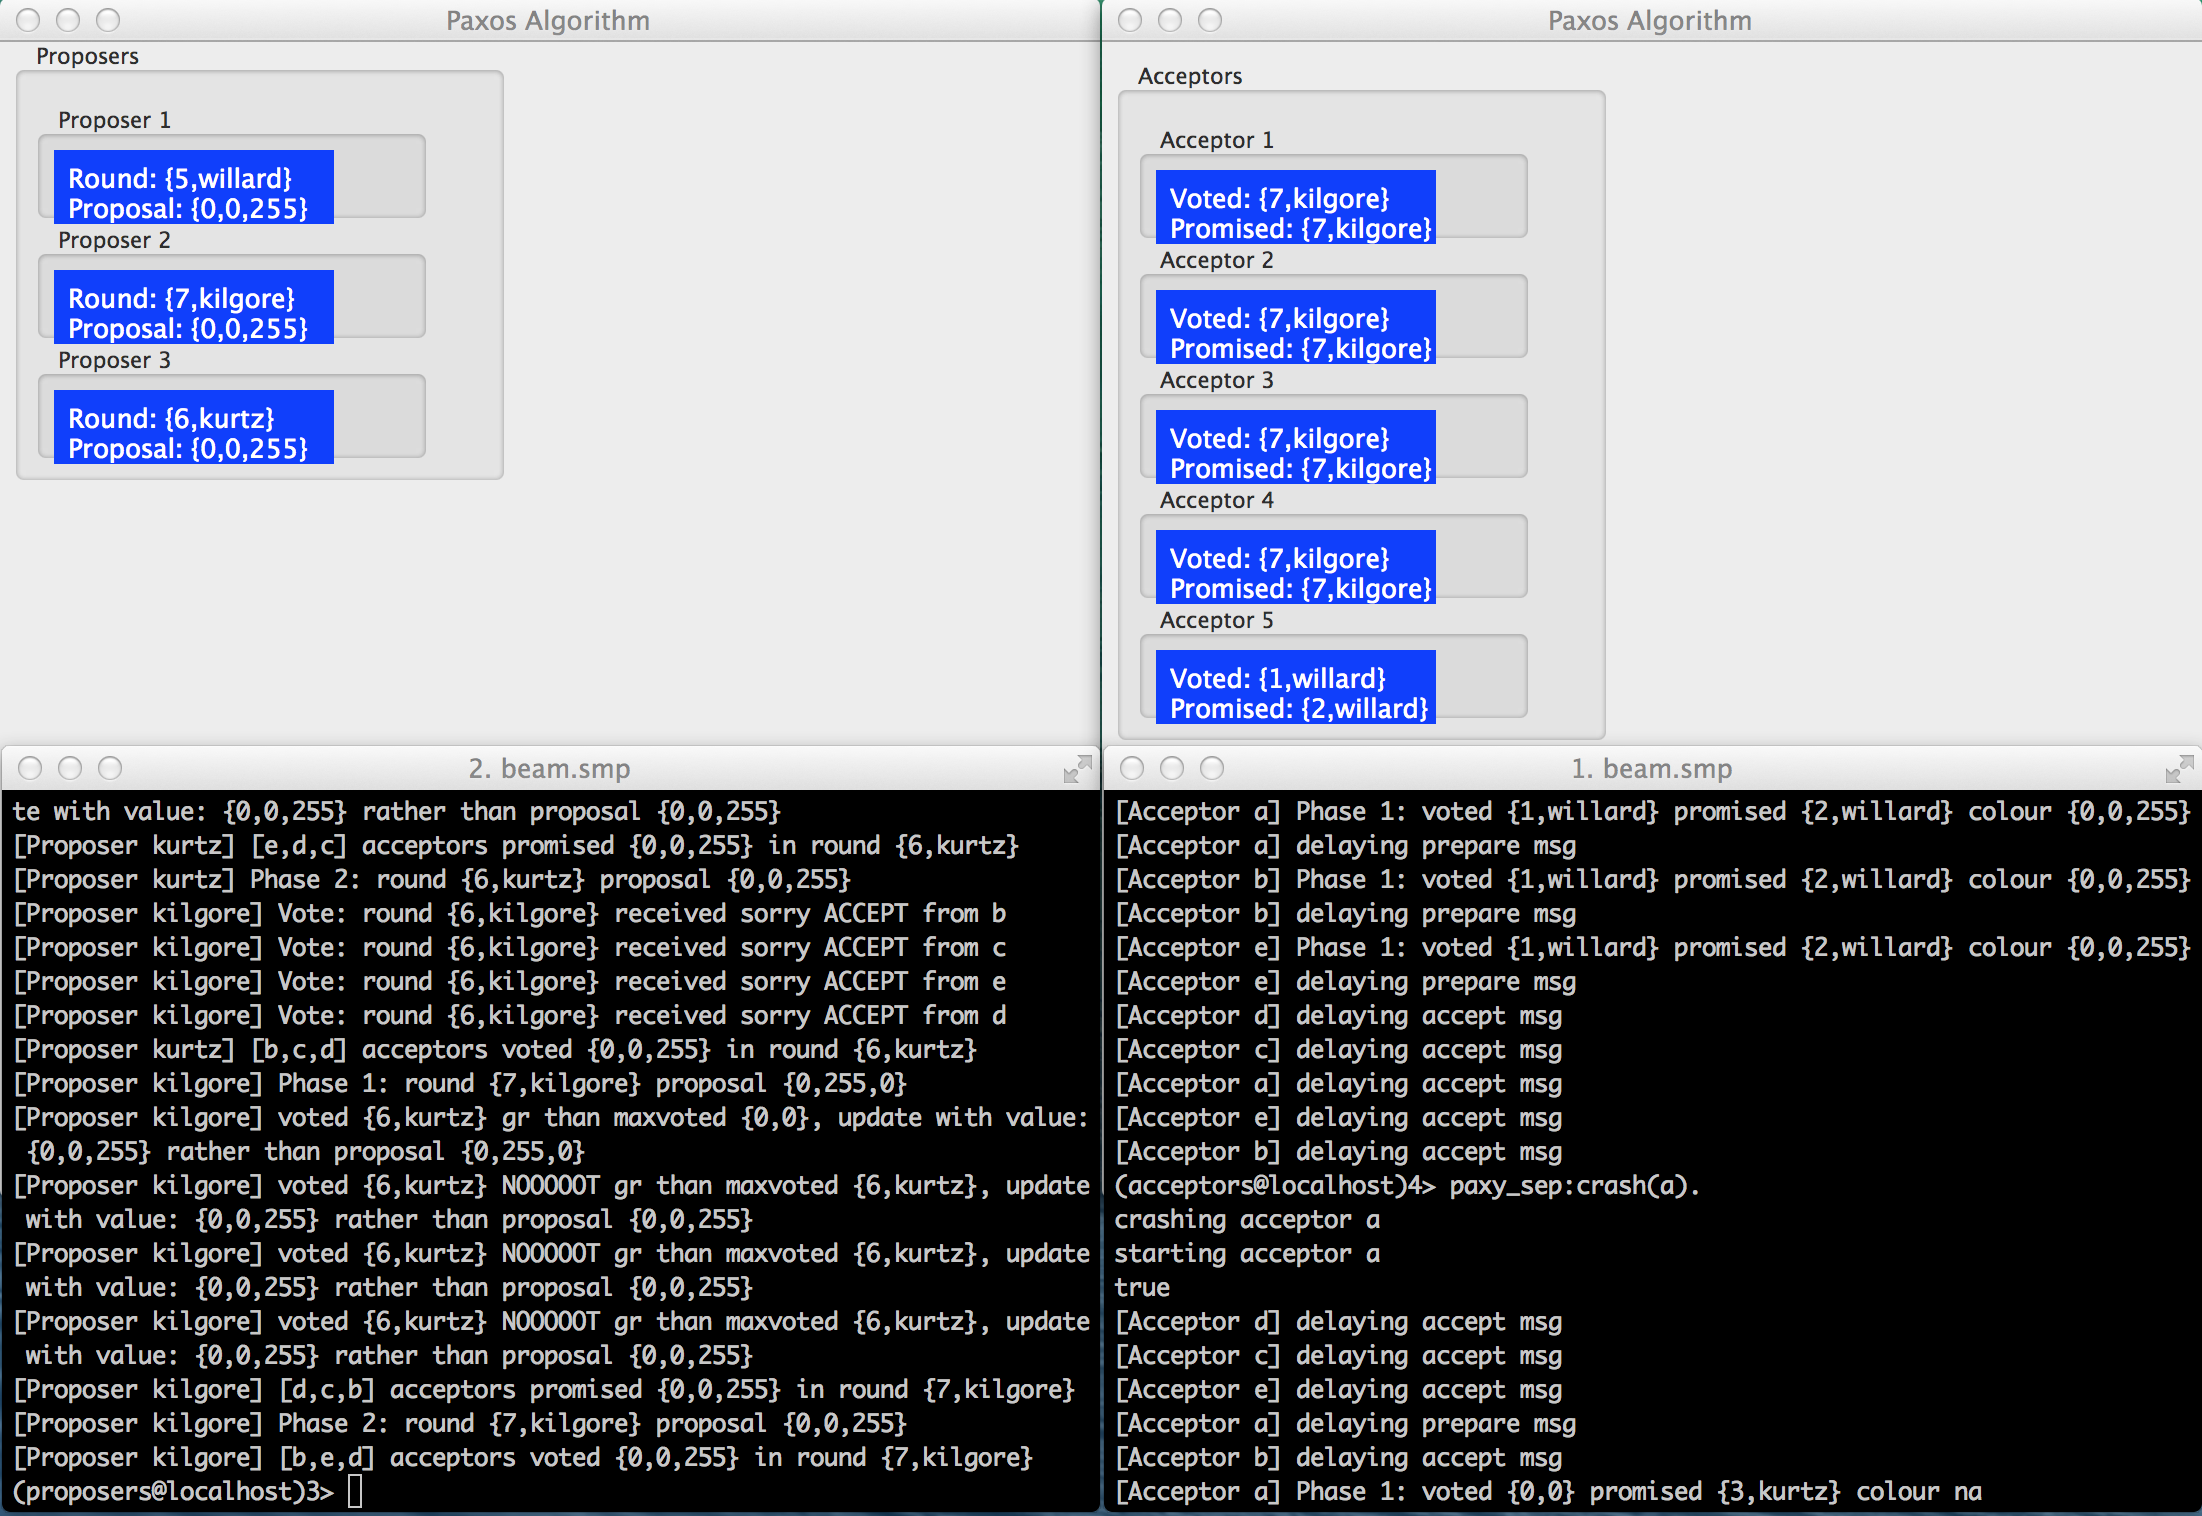
\includegraphics[scale=0.35]{images/exp11.png} \\\\

\textbf{Improvements}
With five acceptors, a proposal needs to be voted on at least 3 times. We changed the \textit{collect} and \textit{vote} functions in the proposer, such that once it receives 3 \textit{sorry} messages it aborts for this proposal. In the experiments trace we see the count of the \textit{sorry} messages and the moment it aborts.\\
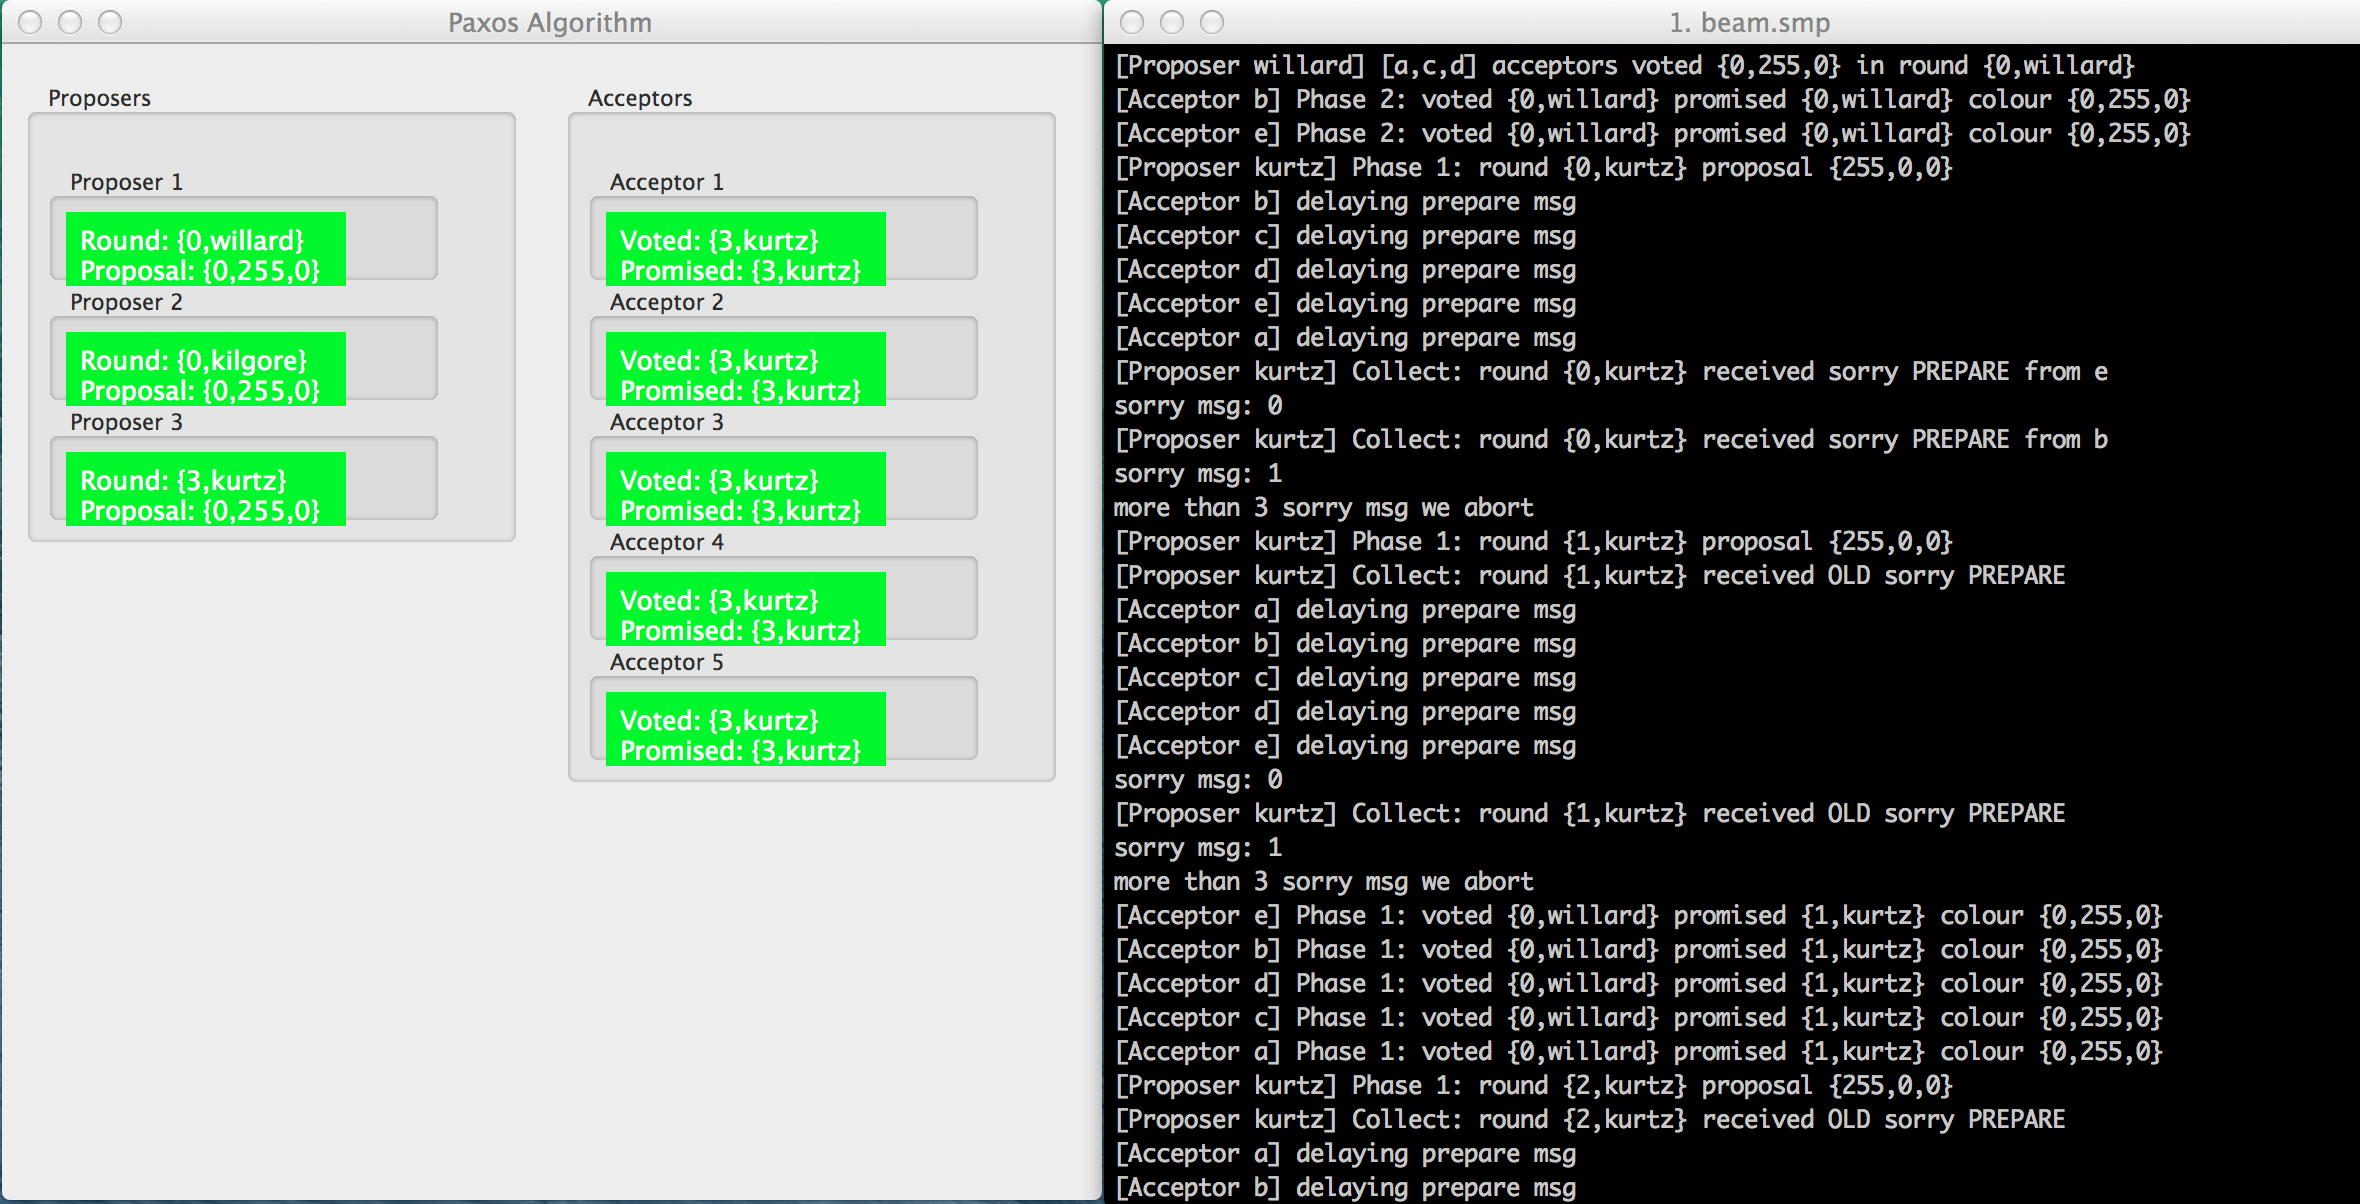
\includegraphics[scale=0.35]{images/exp12.png} \\\\

\section{Personal opinion}

The seminar had the right level of difficulty for this course and the amount of time available to us. We also got a broader understanding of the Paxos algorithm and we managed to run it in a distributed system as well. In our opinion, the seminar should appear in the next year's curriculum.

\end{document}
